\section{Modelling of the Traction of the Metallic Strip}
As presented in the introduction, we know from a physical intuition that the traction in the metallic strip depends mainly on the difference of speed between the rolls, rather than on each of the speeds individually. For this reason, we only have to determine $Trac(s)$ as described in figure \ref{fig:tractionInput}, where $\omega_i$ is the speed of a motor, and $f$ is the traction of the metallic strip\footnote{Since we do not control the middle pair of rolls, we are not able to control the left and right traction separately. For this reason, in the following, we only care about controlling the right traction, which is denoted $f$ but sometimes $f_R$ in the matlab figures. With this setup, the left traction has roughly the same evolution as the right traction, multiplied by a coefficient slightly lower than $1$.}.
\begin{figure}[htbp]
\centering
\begin{tikzpicture}[auto, node distance=2cm,>=latex']
    % We start by placing the blocks
    \node [sum] (sum) {};
    \node [input, left of = sum, yshift = 1cm] (vr) {};
    \node [input, left of = sum, yshift = -1cm](vl) {};
    \node [sum, right of = sum, xshift = 1cm](addspeedsetpoint){};
    \node [input, below of = addspeedsetpoint](speed0){};
    \node [block, right of = addspeedsetpoint, xshift = 1cm](strip){$Trac(s)?$};
    \node [sum, right of = strip, xshift = 2cm](addtracsetpoint){};
    \node [input, below of = addtracsetpoint](tracsetpoint){};
    \node [output, right of = addtracsetpoint](trac){};

    % Once the nodes are placed, connecting them is easy.
    \draw [draw,->] (vr) node [yshift = 3mm]{$\omega_R$} -| node [pos = 0.9]{$+$} (sum);
    \draw [draw,->] (vl) node [yshift = 3mm]{$\omega_L$} -| node [pos = 0.9]{$-$} (sum);
    \draw [draw,->] (sum) -- node {$\Delta_\omega$} node[pos = 0.9]{$+$}  (addspeedsetpoint);
    \draw [draw,->] (speed0) -- node{${\Delta_\omega}_0$} node [pos = 0.9, right]{$-$} (addspeedsetpoint);
    \draw [draw,->]  (addspeedsetpoint) -- node{${\tilde{\Delta_\omega}}$} (strip);
    \draw [draw,->] (strip) -- node {$\tilde{f}$} node[pos = 0.9]{$+$} (addtracsetpoint);
    \draw [draw,->] (tracsetpoint) -- node {$f_0$} node[pos = 0.9, right]{$+$} (addtracsetpoint);
    \draw [draw,->] (addtracsetpoint) -- node {$f$} (trac);

\end{tikzpicture}
\caption{\label{fig:tractionInput}Simple gray-box model of the traction of the metallic strip}
\end{figure}

Furthermore, we also know that $Trac(s)$ should contain a close-to-perfect integrator. Indeed, if we increase $\Delta_\omega$ slightly from the setpoint ${\Delta_\omega}_0$, we expect the tension in the metallic strip to rise indefinitely until breakage. This is also confirmed by the experience: we observe that the system's response to a real world pulse is really close to a step, as showed in figure \ref{fig:tracImpulseResponse}.
\begin{figure}[htbp]
\centering
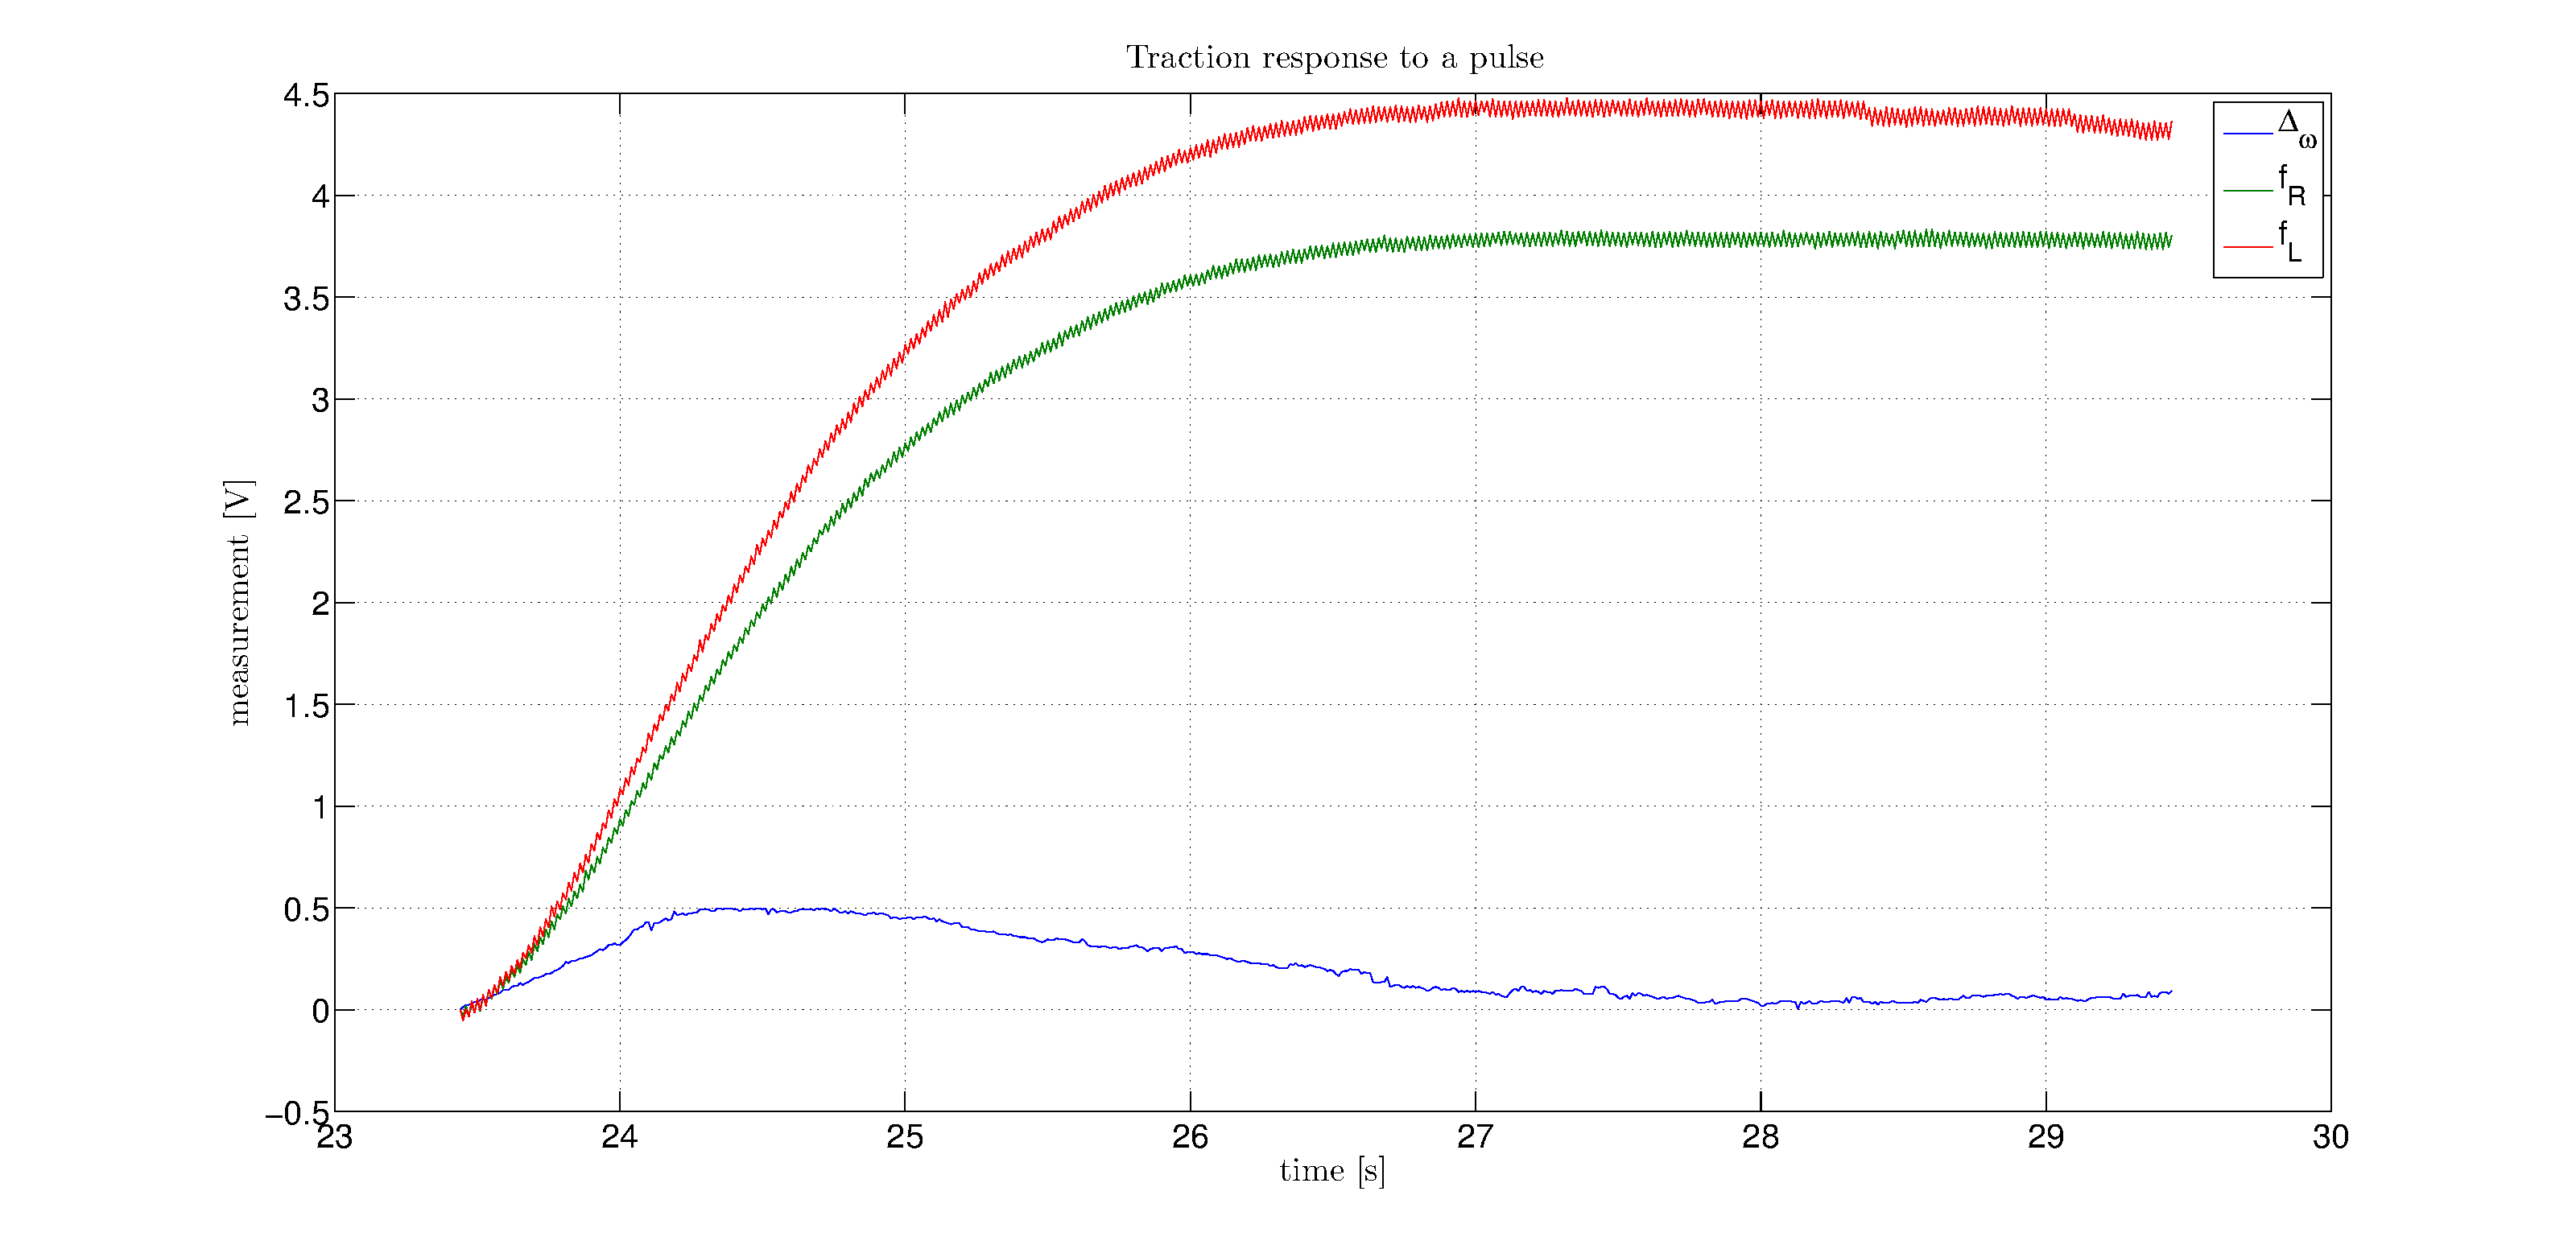
\includegraphics[width = \textwidth]{tractionPulse.pdf}
\caption{Traction response to a real world pulse\label{fig:tracImpulseResponse}}
\end{figure}
Finally, this is supported by a second order numerical approximation of the dynamics, which always yields a pole that is very close to zero.

However, this leads the rest of the optimisation problem to be badly conditioned. This means that the second pole is not reliably placed, and that the final result does not fit the real response accurately. Moreover, the obtained transfer function, with a very large $K$ and $p_2$, takes a long time to simulate with simulink.

To solve this, we refine our gray-box approximation by artificially introducing an integrator in the system we want to identify. We then compute its response to $\tilde{\Delta_\omega}(t)$ and try to determine the rest of the dynamics based on this new input and the observed response, as shown in figure \ref{fig:tractionGrayBox}, where $\frac{1}{s}\cdot H(s) = Trac(s)$. In the figure, we also use the fact that only $\omega_L$ is supposed to contribute to $\tilde{\Delta_\omega}$, since the master velocity is chosen steady. $\tilde{\omega_R}$ is thus considered as a disturbance.
\begin{figure}[htbp]
\centering
\begin{tikzpicture}[auto, node distance=2cm,>=latex']
    % We start by placing the blocks
    \node [input](input){};
    \node [sum, right of = input, xshift = 0.5cm](add){};
    \node [input, above of = add, yshift = -0.8cm](disturb){};
    \node [square, right of = add, xshift = 0cm](integrator){$\frac{1}{s}$};
    \node [block, right of = integrator, xshift = 2.5cm](strip){$H(s)?$};
    \node [output, right of = strip](trac){};

    % Once the nodes are placed, connecting them is easy.
    \draw [draw,->]  (input) -- node{${\tilde{\omega_L}}$} node[pos = 0.9, below]{$-$} (add);
    \draw [draw,->]  (disturb) -- node[pos = 0.2]{$d$} node[pos = 0.9]{$+$} (add);
    \draw [draw,->]  (add) -- (integrator);
    \draw [draw,->]  (integrator) -- node{${\int^t_0\tilde{\omega_L}}dt$} (strip);
    \draw [draw,->] (strip) -- node {$\tilde{f}$} (trac);
\end{tikzpicture}
\caption{Gray-box model of the traction of the metallic strip\label{fig:tractionGrayBox}}
\end{figure}

Fitting a simple first order transfer function to $H(s)$ is not easy because the dynamics between $\int_0^t\tilde{\omega_L}(t)$ and $f(t)$ is very fast, as shown in figure \ref{fig:tractionPulseStep}. This leads to very large poles which are not well approximated and difficult to simulate, as experienced previously.
\begin{figure}[htbp]
\centering
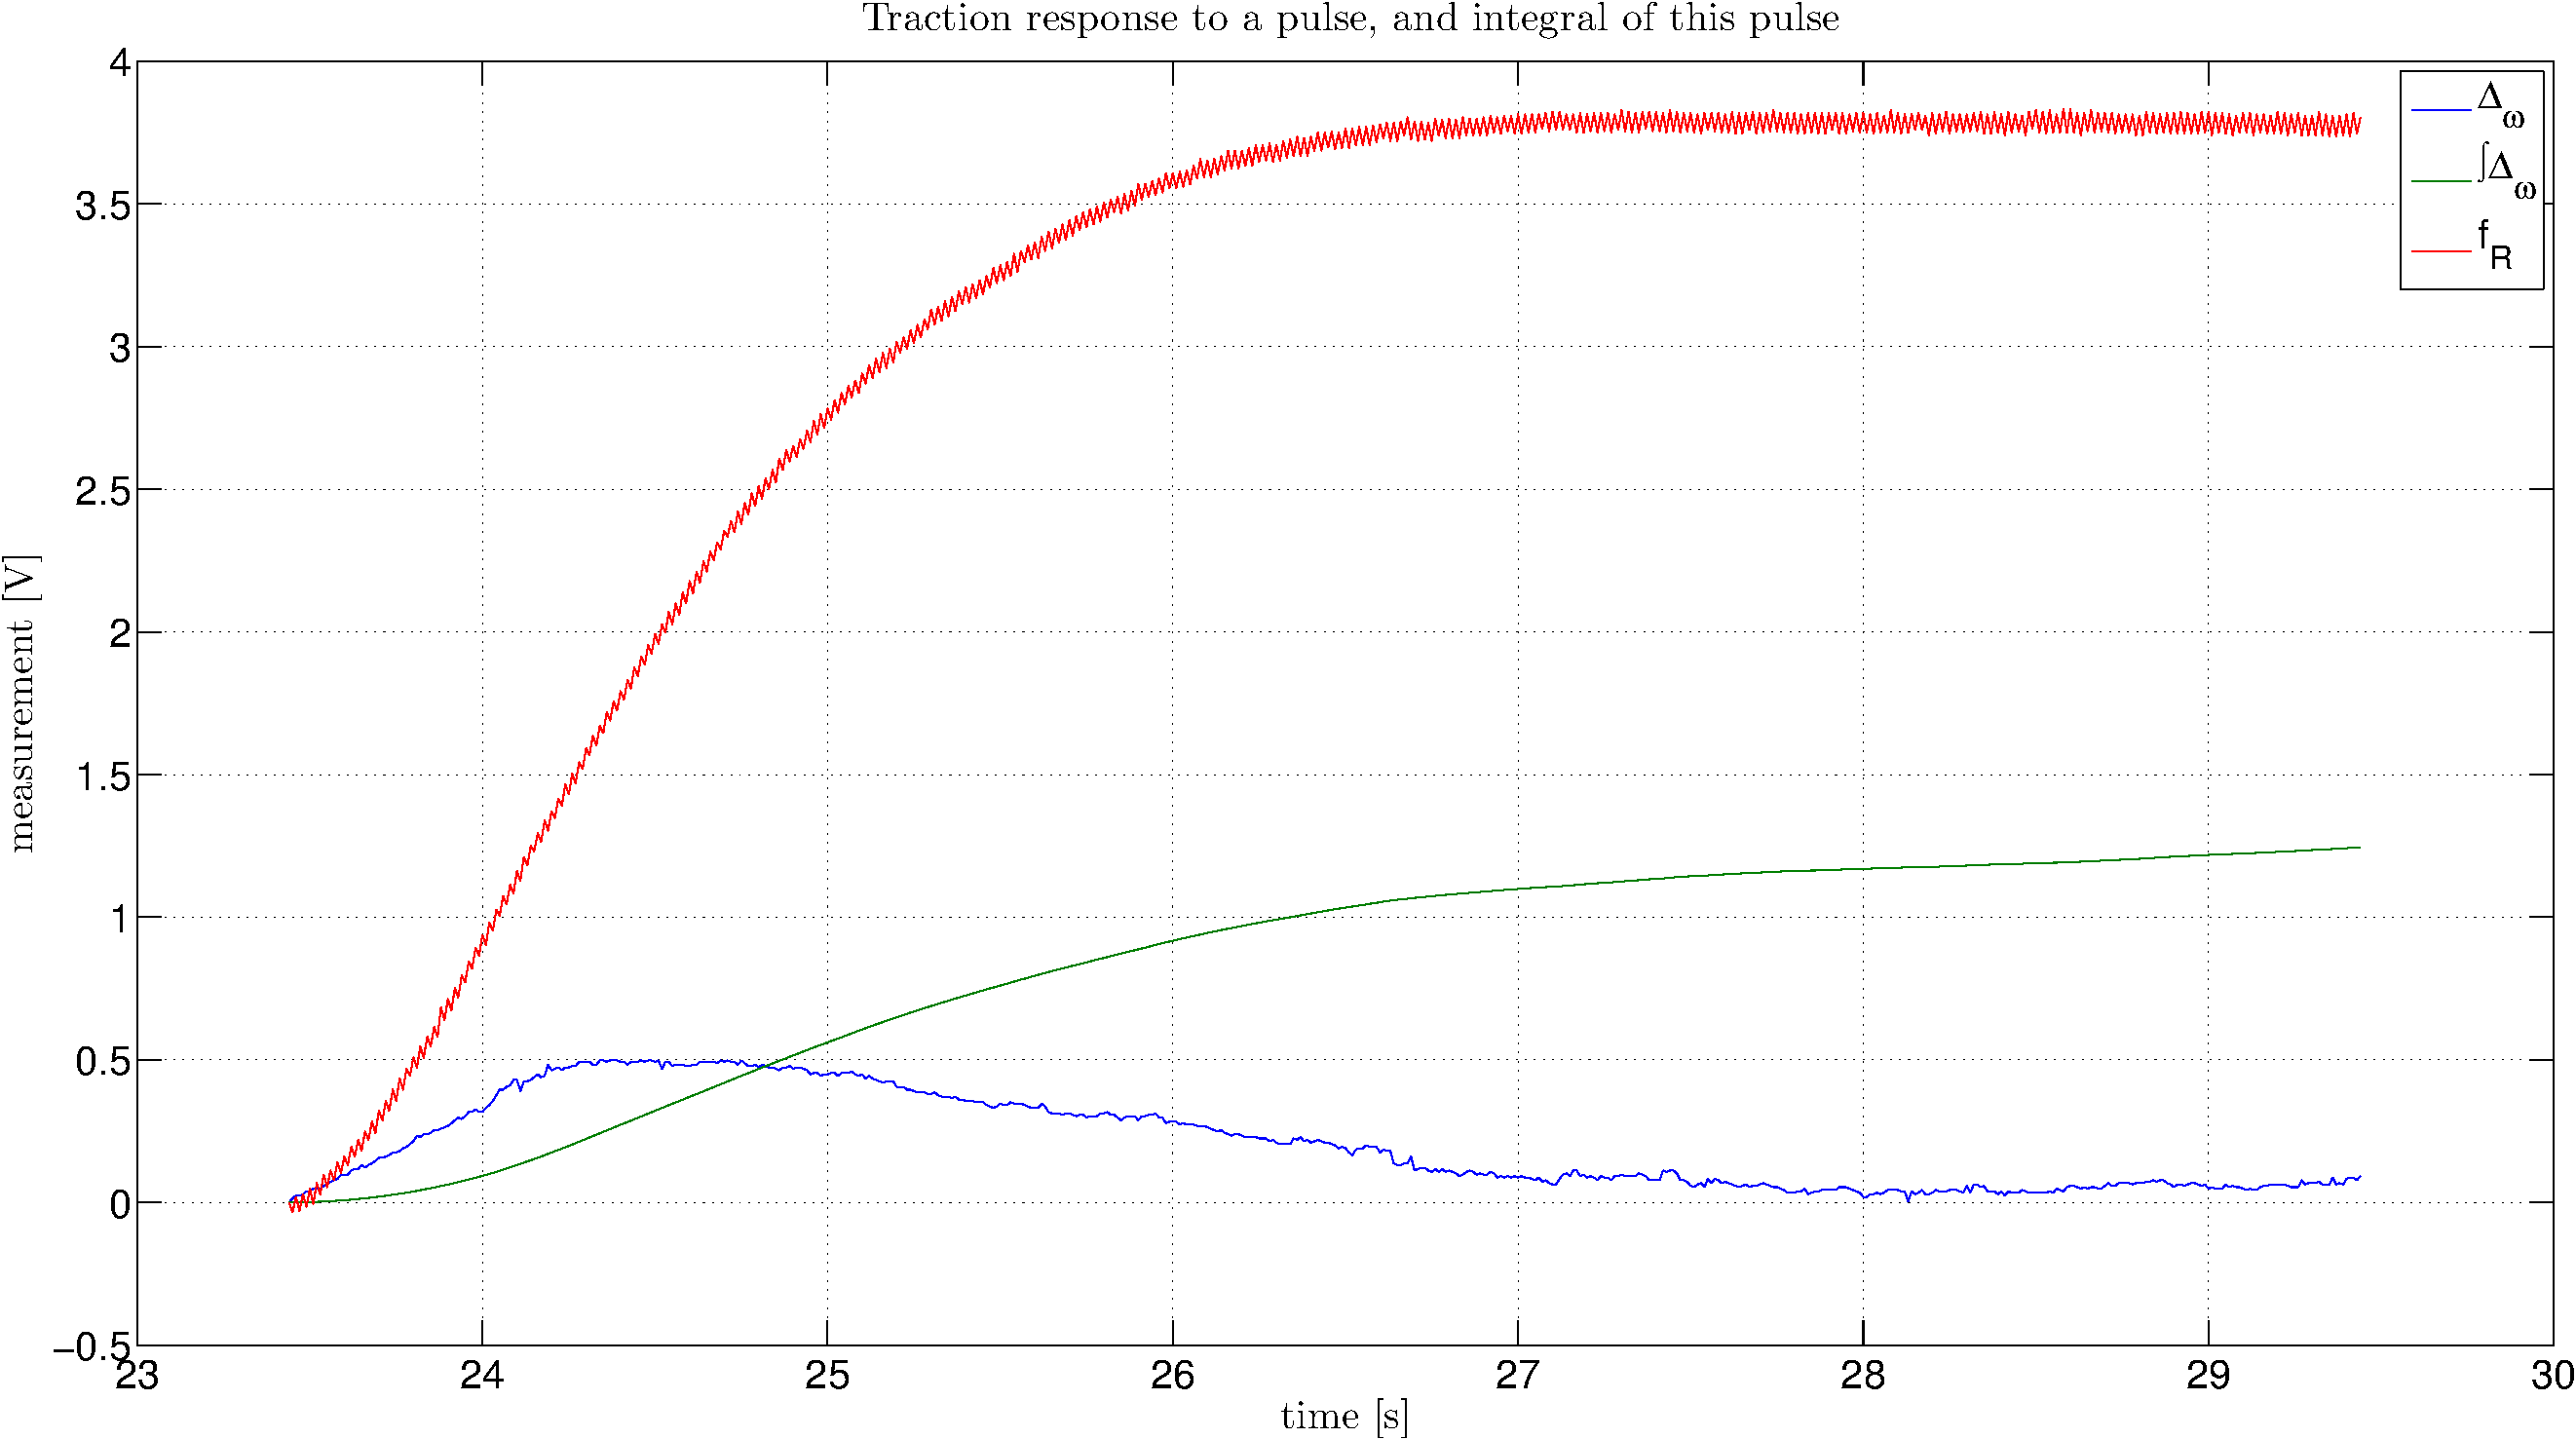
\includegraphics[width = \textwidth]{tractionPulseStep.pdf}
\caption{Right traction response to a pulse and output of the intermediate integrator\label{fig:tractionPulseStep}}
\end{figure}

To solve this, we try to fit $H(s)$ with a transfer function of the form $K\frac{s-z_1}{s-p_2}$, because the introduction of a zero speeds up a step response, which would bring $p_2$ reasonably closer to the origin. The result is shown in figure \ref{fig:tracFit}, where we see that $Trac(s)$ as given in equation \ref{eqn:tracS} seems to fit the experience very well.
\begin{align*}
  H(s) &= 13.096\cdot\frac{s+0.9221}{s+4.063}\\
  Trac(s) &= 13.096\cdot\frac{s+0.9221}{s(s+4.063)}\numberthis\label{eqn:tracS}
\end{align*}
\begin{figure}[htbp]
\centering
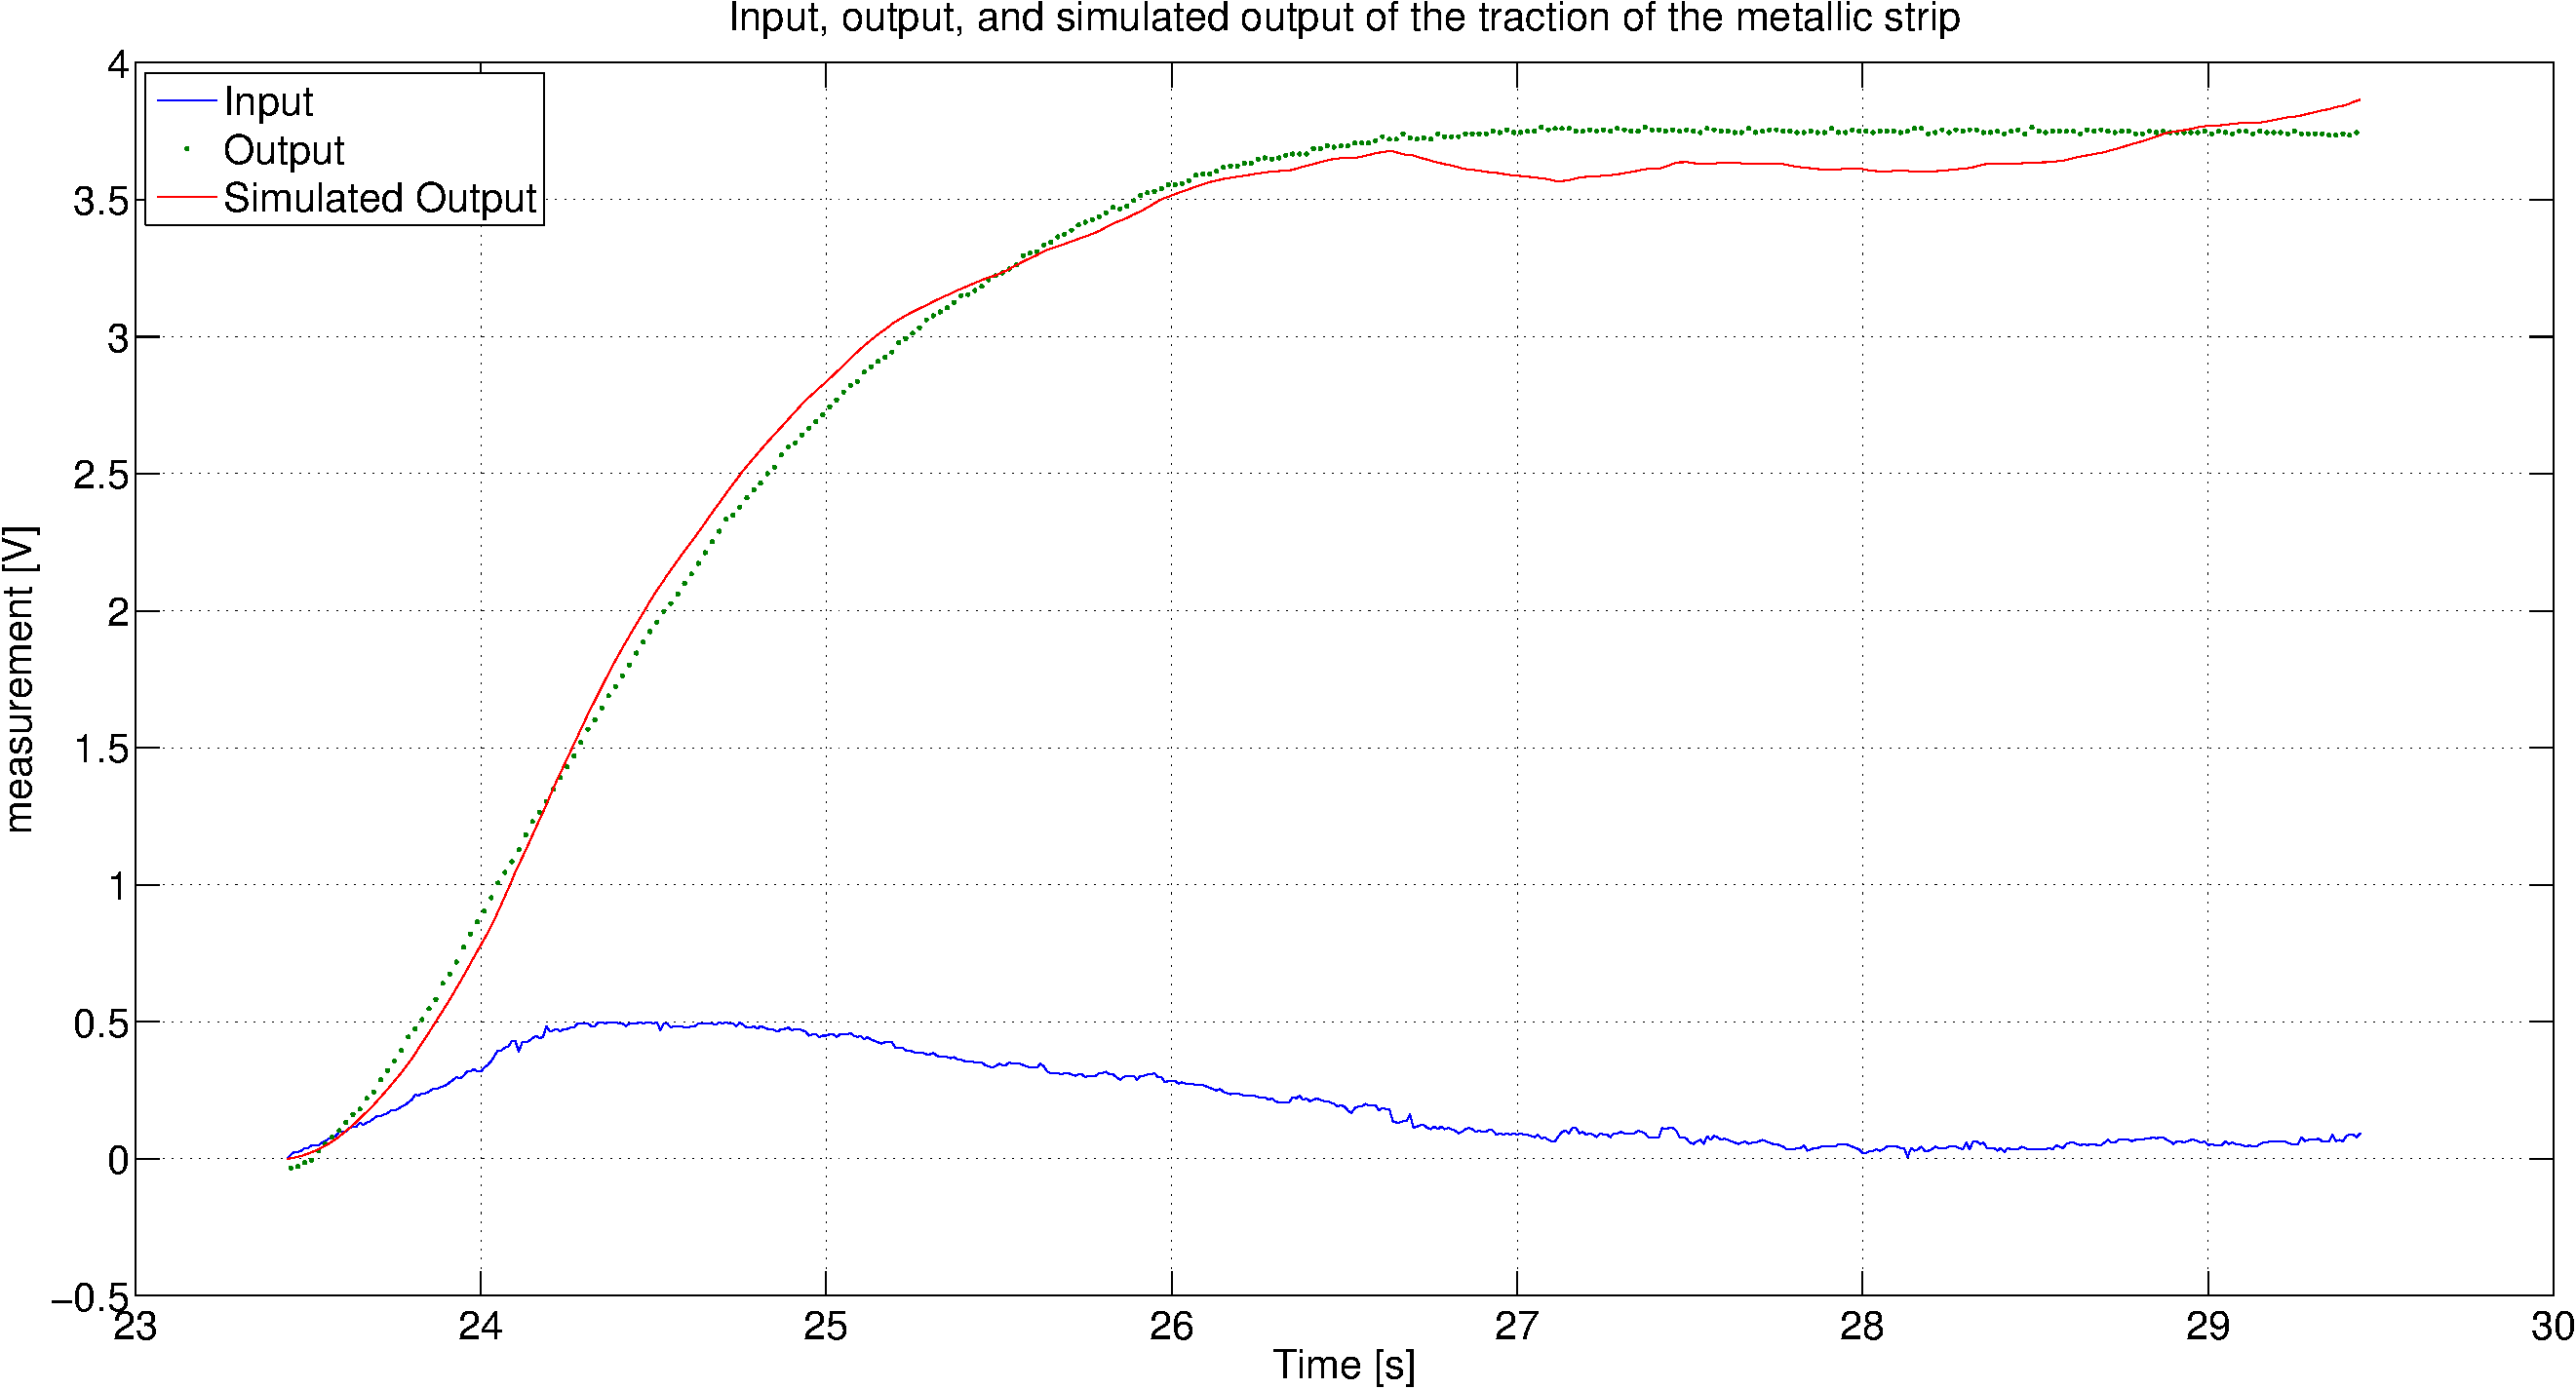
\includegraphics[width = \textwidth]{tracFit.pdf}
\caption{Input, output, and simulated output of the traction of the metallic strip\label{fig:tracFit}}
\end{figure}

\section{Control of the Traction}
\subsection{Simple P Controller}
Since there already is an integrator in the system, and since we do not have specifications on the transient response, we first try to control the traction with a simple P~controller, which should provide asymptotic stability and zero steady-state error. Figure \ref{fig:tracRLocus}
\begin{figure}[htbp]
  \centering
  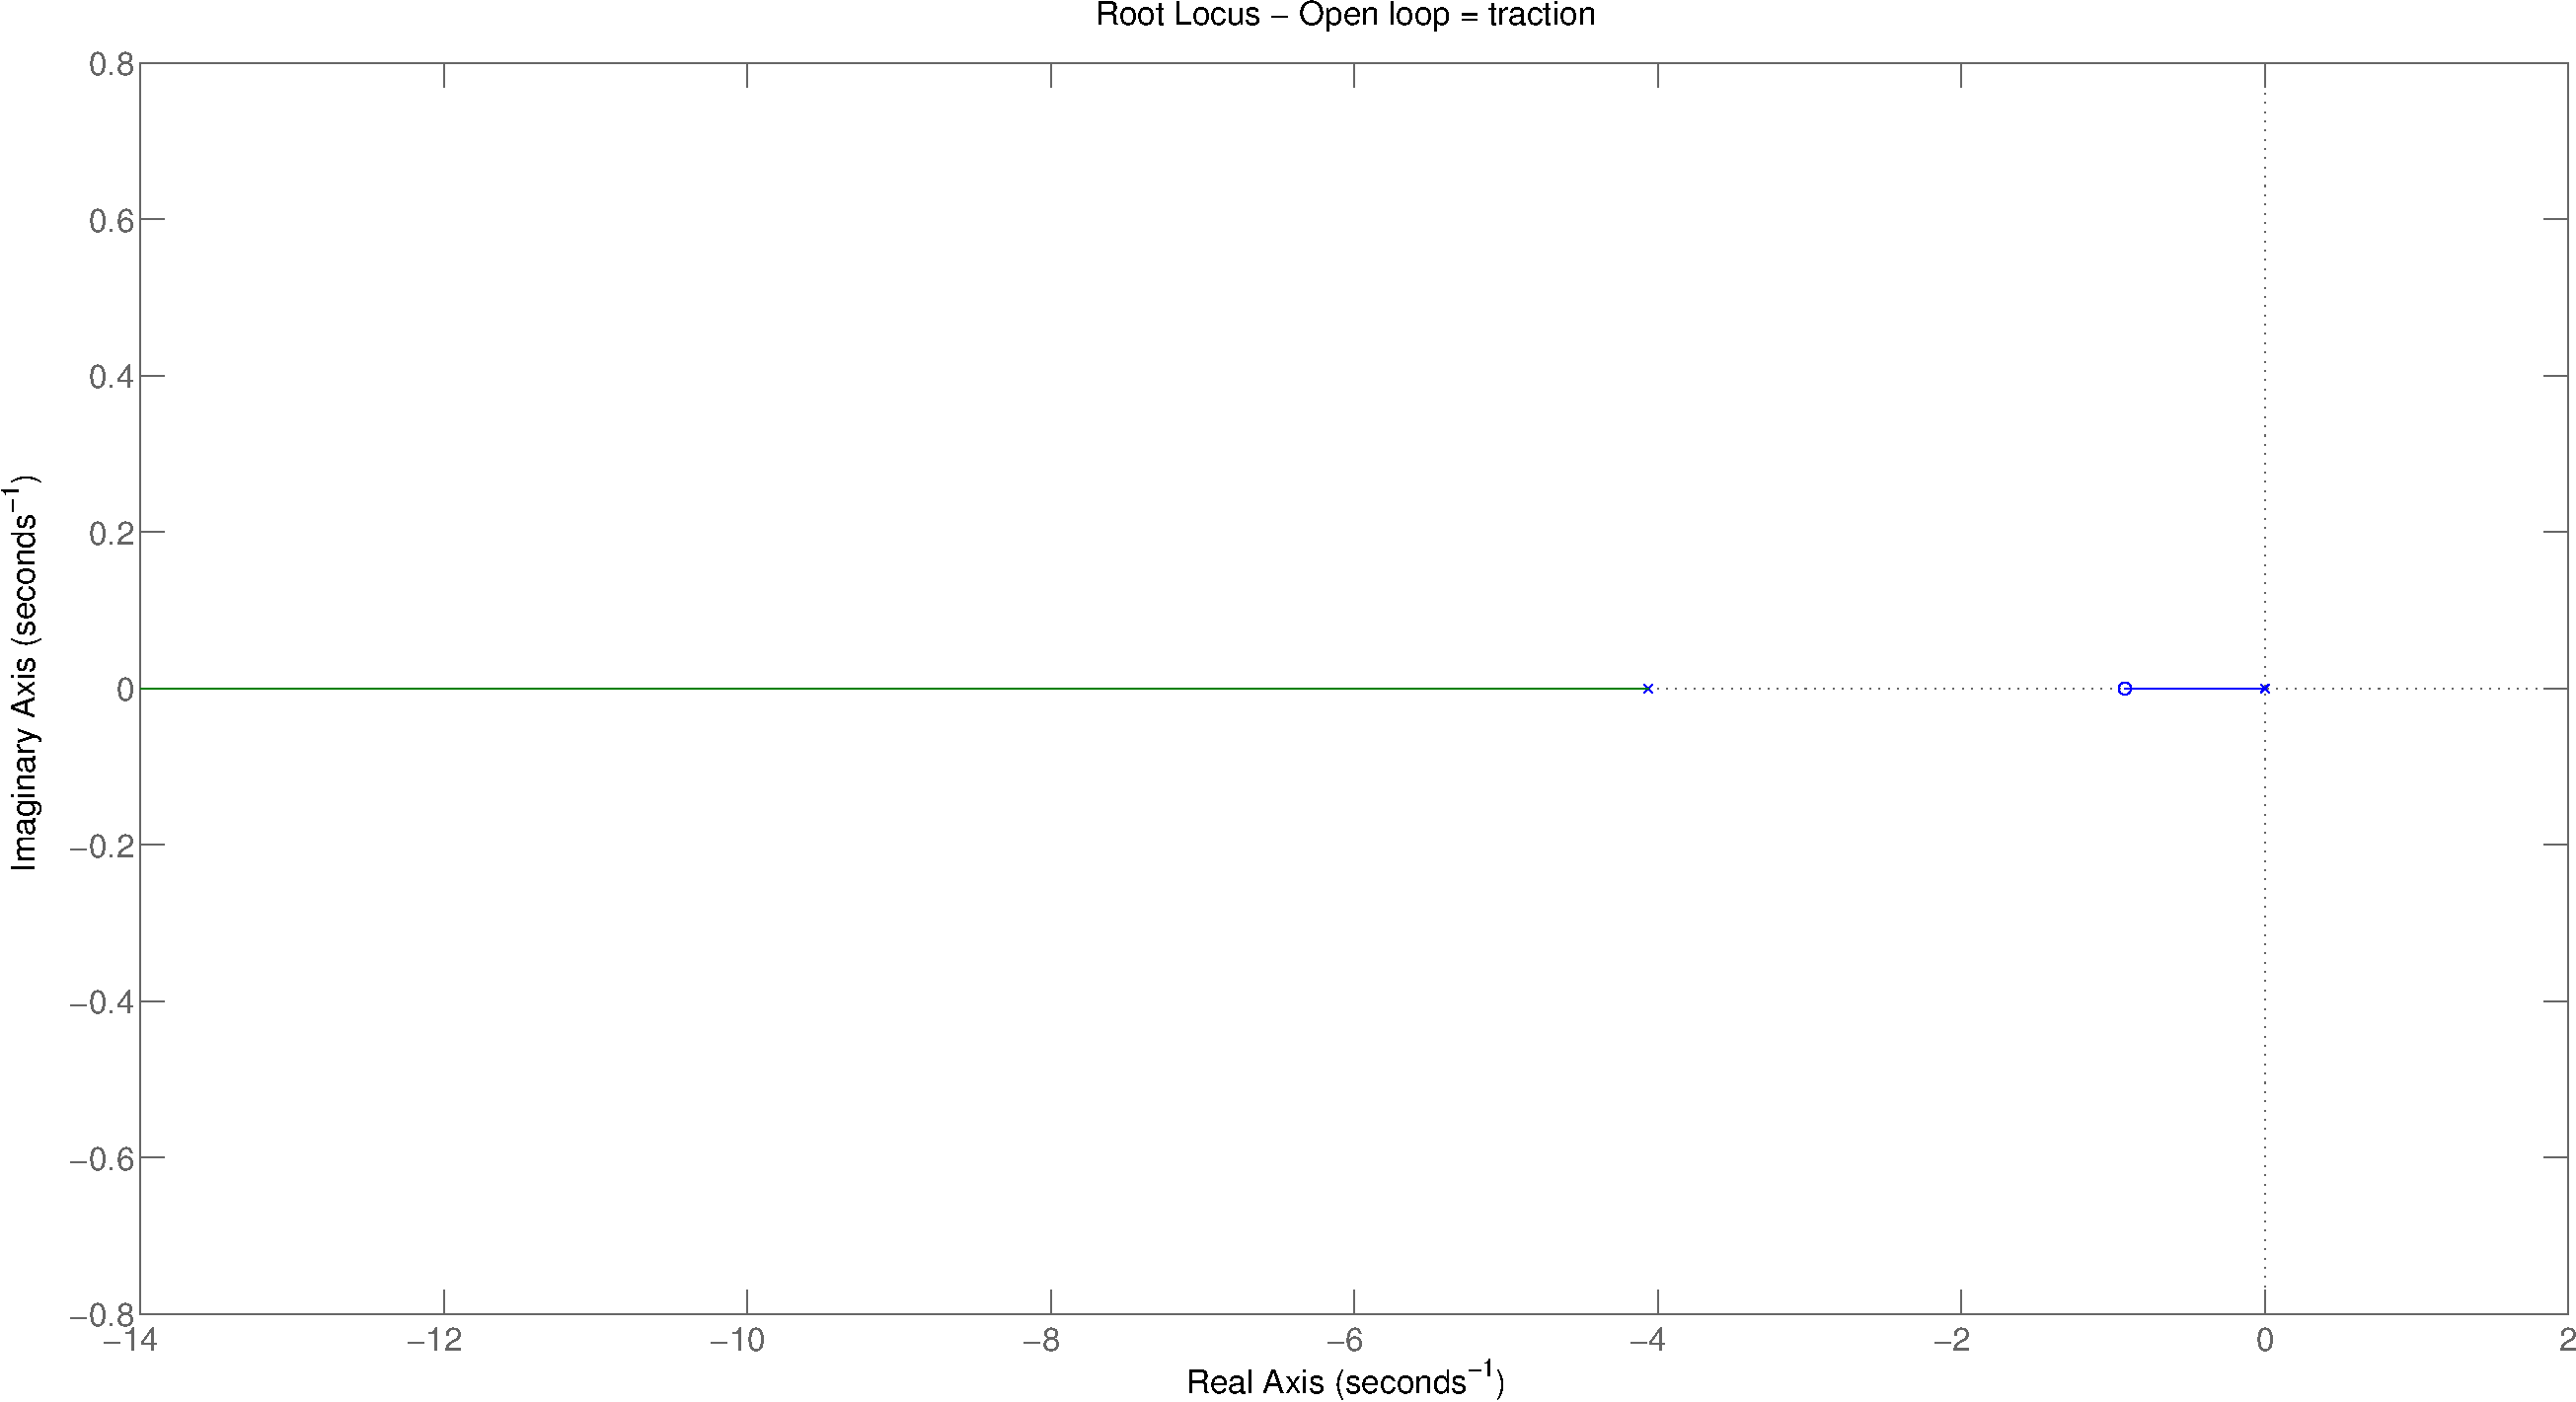
\includegraphics[width = \textwidth]{rlocus_trac.pdf}
  \caption{Root locus of the traction\label{fig:tracRLocus}}
\end{figure}
shows the root locus of the traction for this controller, with the approximation that the inner slave speed loop is fast enough to be considered perfectly transparent. The root locus shows that $k_P < 0$\footnote{The $\tilde{\omega_L}$ input is inverting, as shown in figure \ref{fig:tractionGrayBox}} can be theoretically chosen as high as desired while keeping the closed-loop poles on the real axis.

Figure \ref{fig:simuPTot}
\begin{figure}[htbp]
  \centering
  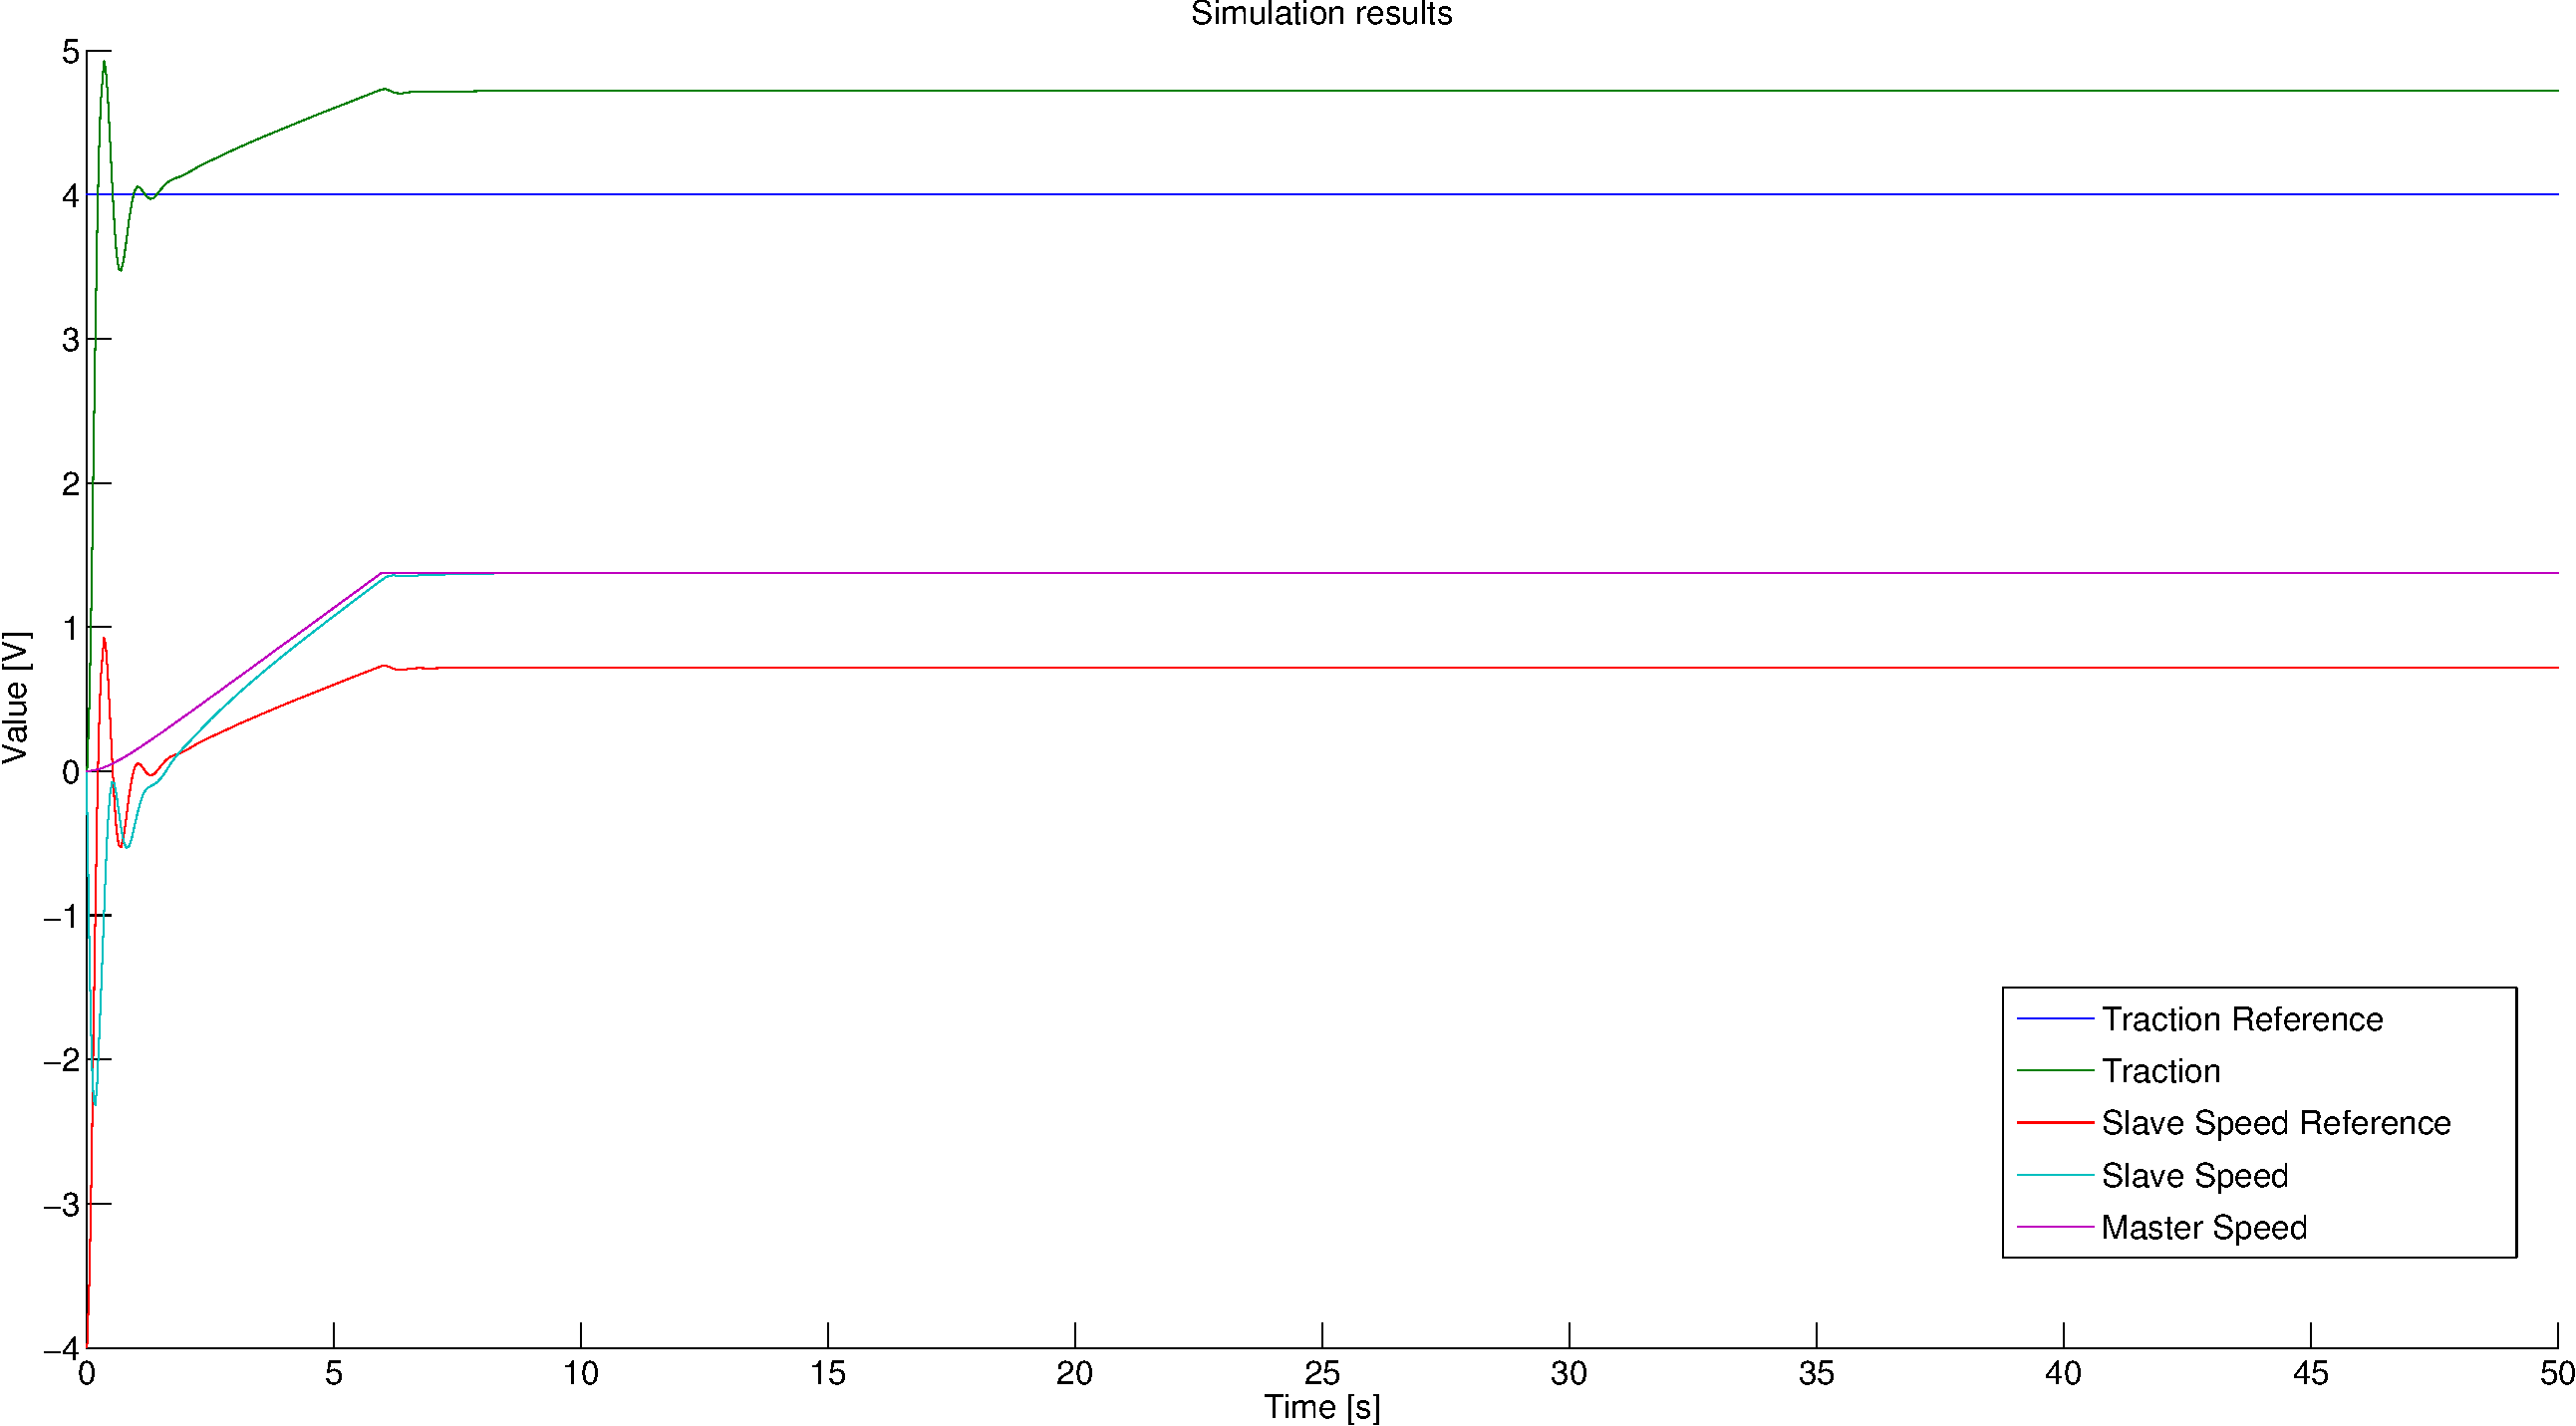
\includegraphics[width = \textwidth]{simu_P_tot.pdf}
  \caption{Simulation of the rolling mill operation with a P controller on the traction\label{fig:simuPTot}}
\end{figure}
shows the closed-loop traction response to a constant reference, with an arbitrary gain of $-1$, as simulated by simulink. First, we observe that the closed-loop poles are not real, which is due to non linearities and higher order effects. More importantly, we see that the steady-state error is not cancelled.

Comparing the measured traction and the master speed, we observe that the initial ramp on the master motor is not compensated. In steady state, the master speed also creates an offset on the traction. This is because the right velocity is actually a disturbance, as was shown in figure \ref{fig:tractionGrayBox}. This disturbance is not rejected because the integrator is in the plant, and not in the controller.

To achieve perturbation rejection, an integrator should be added to the controller. However, this is not a good solution as is, because the open loop would then contain two integrators. This would greatly reduce the phase margin and thus make the closed loop system nearly unstable and slow its response down.

\subsection{Second Loop: PI Controller}
Rather then adding an integrator to the existing controller, we can add a second external loop with a PI, as shown in figure \ref{fig:simulinkTot}
\begin{figure}[htbp]
  \centering
  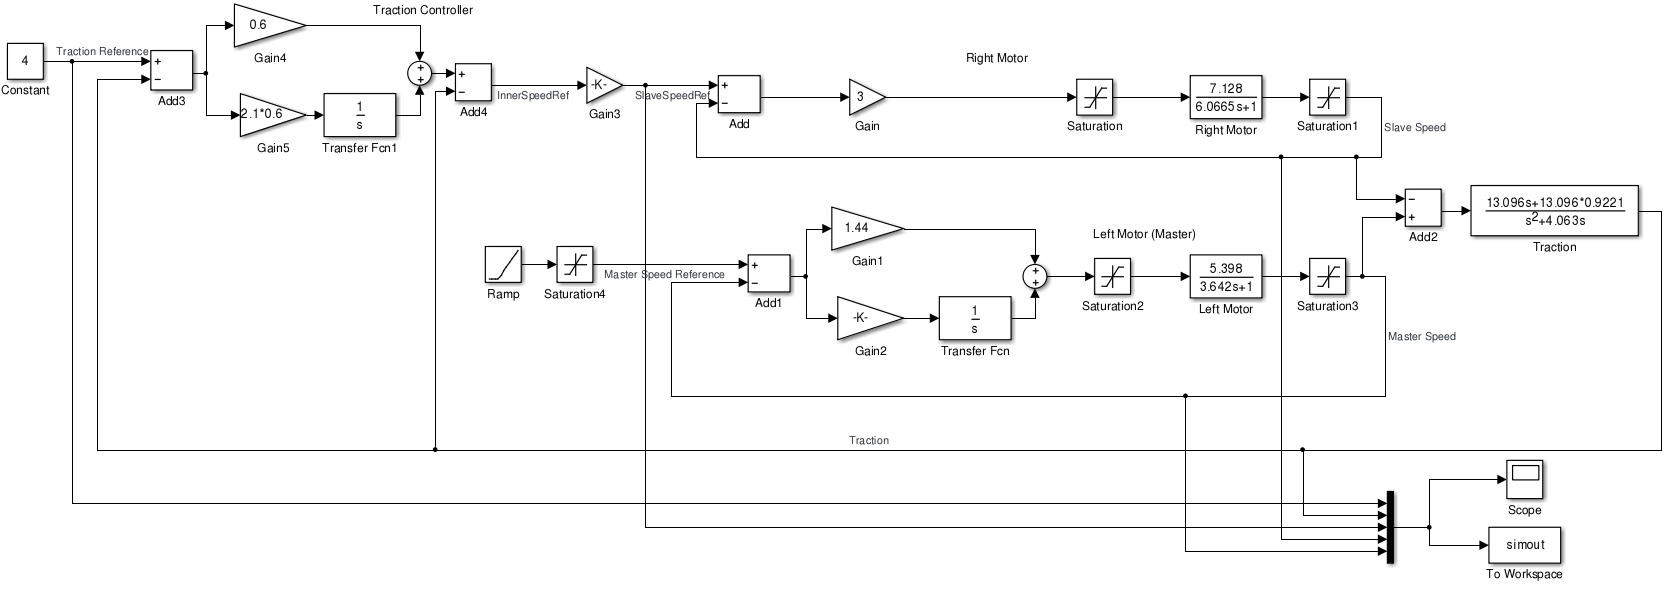
\includegraphics[width = \textwidth]{simulink.png}
  \caption{Final controller architecture\label{fig:simulinkTot}}
\end{figure}
,to achieve perturbation rejection while preserving the phase margin. In this subsection, the reasoning behind this second loop will be explained. In the following, we do not neglect the effect of the inner slave speed loop anymore. However, we do make the approximation that the traction is a essentially an integrator\footnote{Neglecting the higher order zeroes and poles in $Trac(s)$ given in equation~\ref{eqn:tracS}, we obtain $Trac_{approx}(s) = \frac{7.16}{s}$.}. The plant that is controlled using an inner P and an outer PI is thus approximated by the series of the closed loop transfer function of the slave motor and an integrator -- the transfer function of the traction.

With that in mind, the closed loop poles of the inner traction loop are given by figure~\ref{fig:rmTracLocus}
\begin{figure}[htbp]
  \centering
  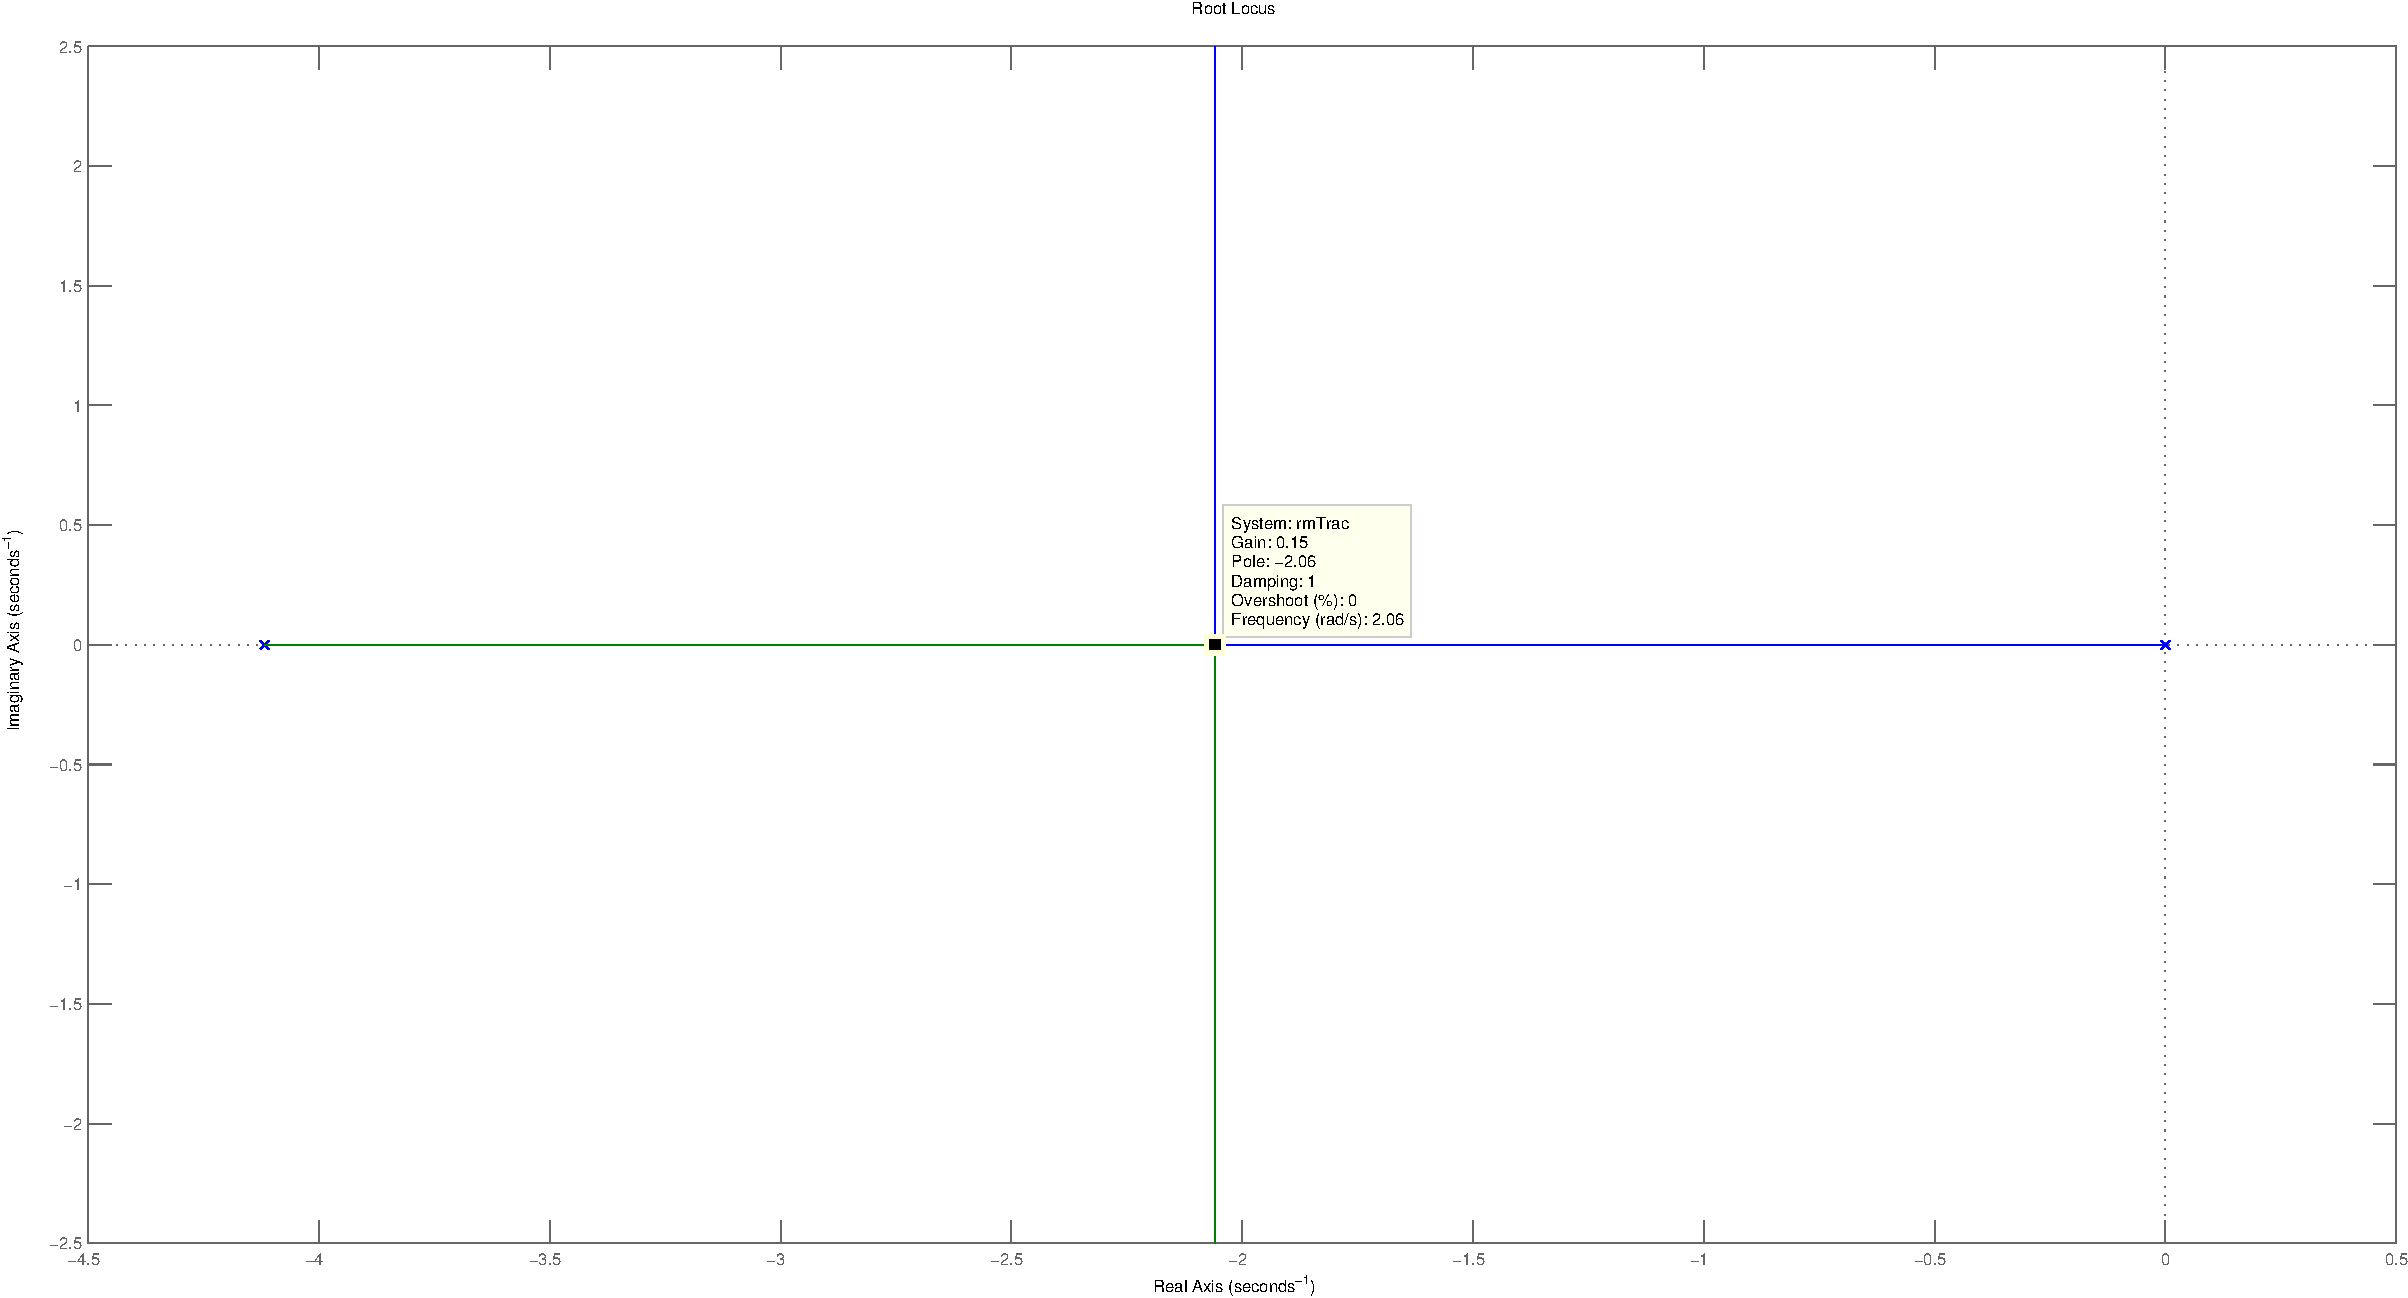
\includegraphics[width = \textwidth]{rmTrac_locus.pdf}
  \caption{Root locus of the inner traction loop\label{fig:rmTracLocus}}
\end{figure}
,which shows the root locus of $Slave(s) \cdot Trac_{approx}(s)$. We observe that using a P controller, it is possible to move the integrator pole into the LHP, which is the essence of feedback control. This is the reason why we can now afford to add a PI outer loop: for an adequate choice of ${K_p}_{inner}$, the plant, which is given by closed loop transfer function of the inner traction loop, can have two real, negative poles. This means that adding a PI to it will ensure a reasonable phase margin, as well as zero steady state error and perturbation rejection.

On figure \ref{fig:rmTracLocus} we choose ${K_p}_{inner} \lessapprox 0.15$ to obtain the fastest possible real poles for the inner loop. This yields a pair of real poles around $-2$. There is now left to determine the gains of the outer PI, given those inner loop poles to complete the controller design of our rolling mill.

To do so, we use the classical approach of canceling the slowest pole in the plant with the zero from the PI, and then determining a first ${K_p}_{outer}$ with a root locus. The resulting plot is shown in figure \ref{fig:rlocus_OuterTrac}.
\begin{figure}[htbp]
  \centering
  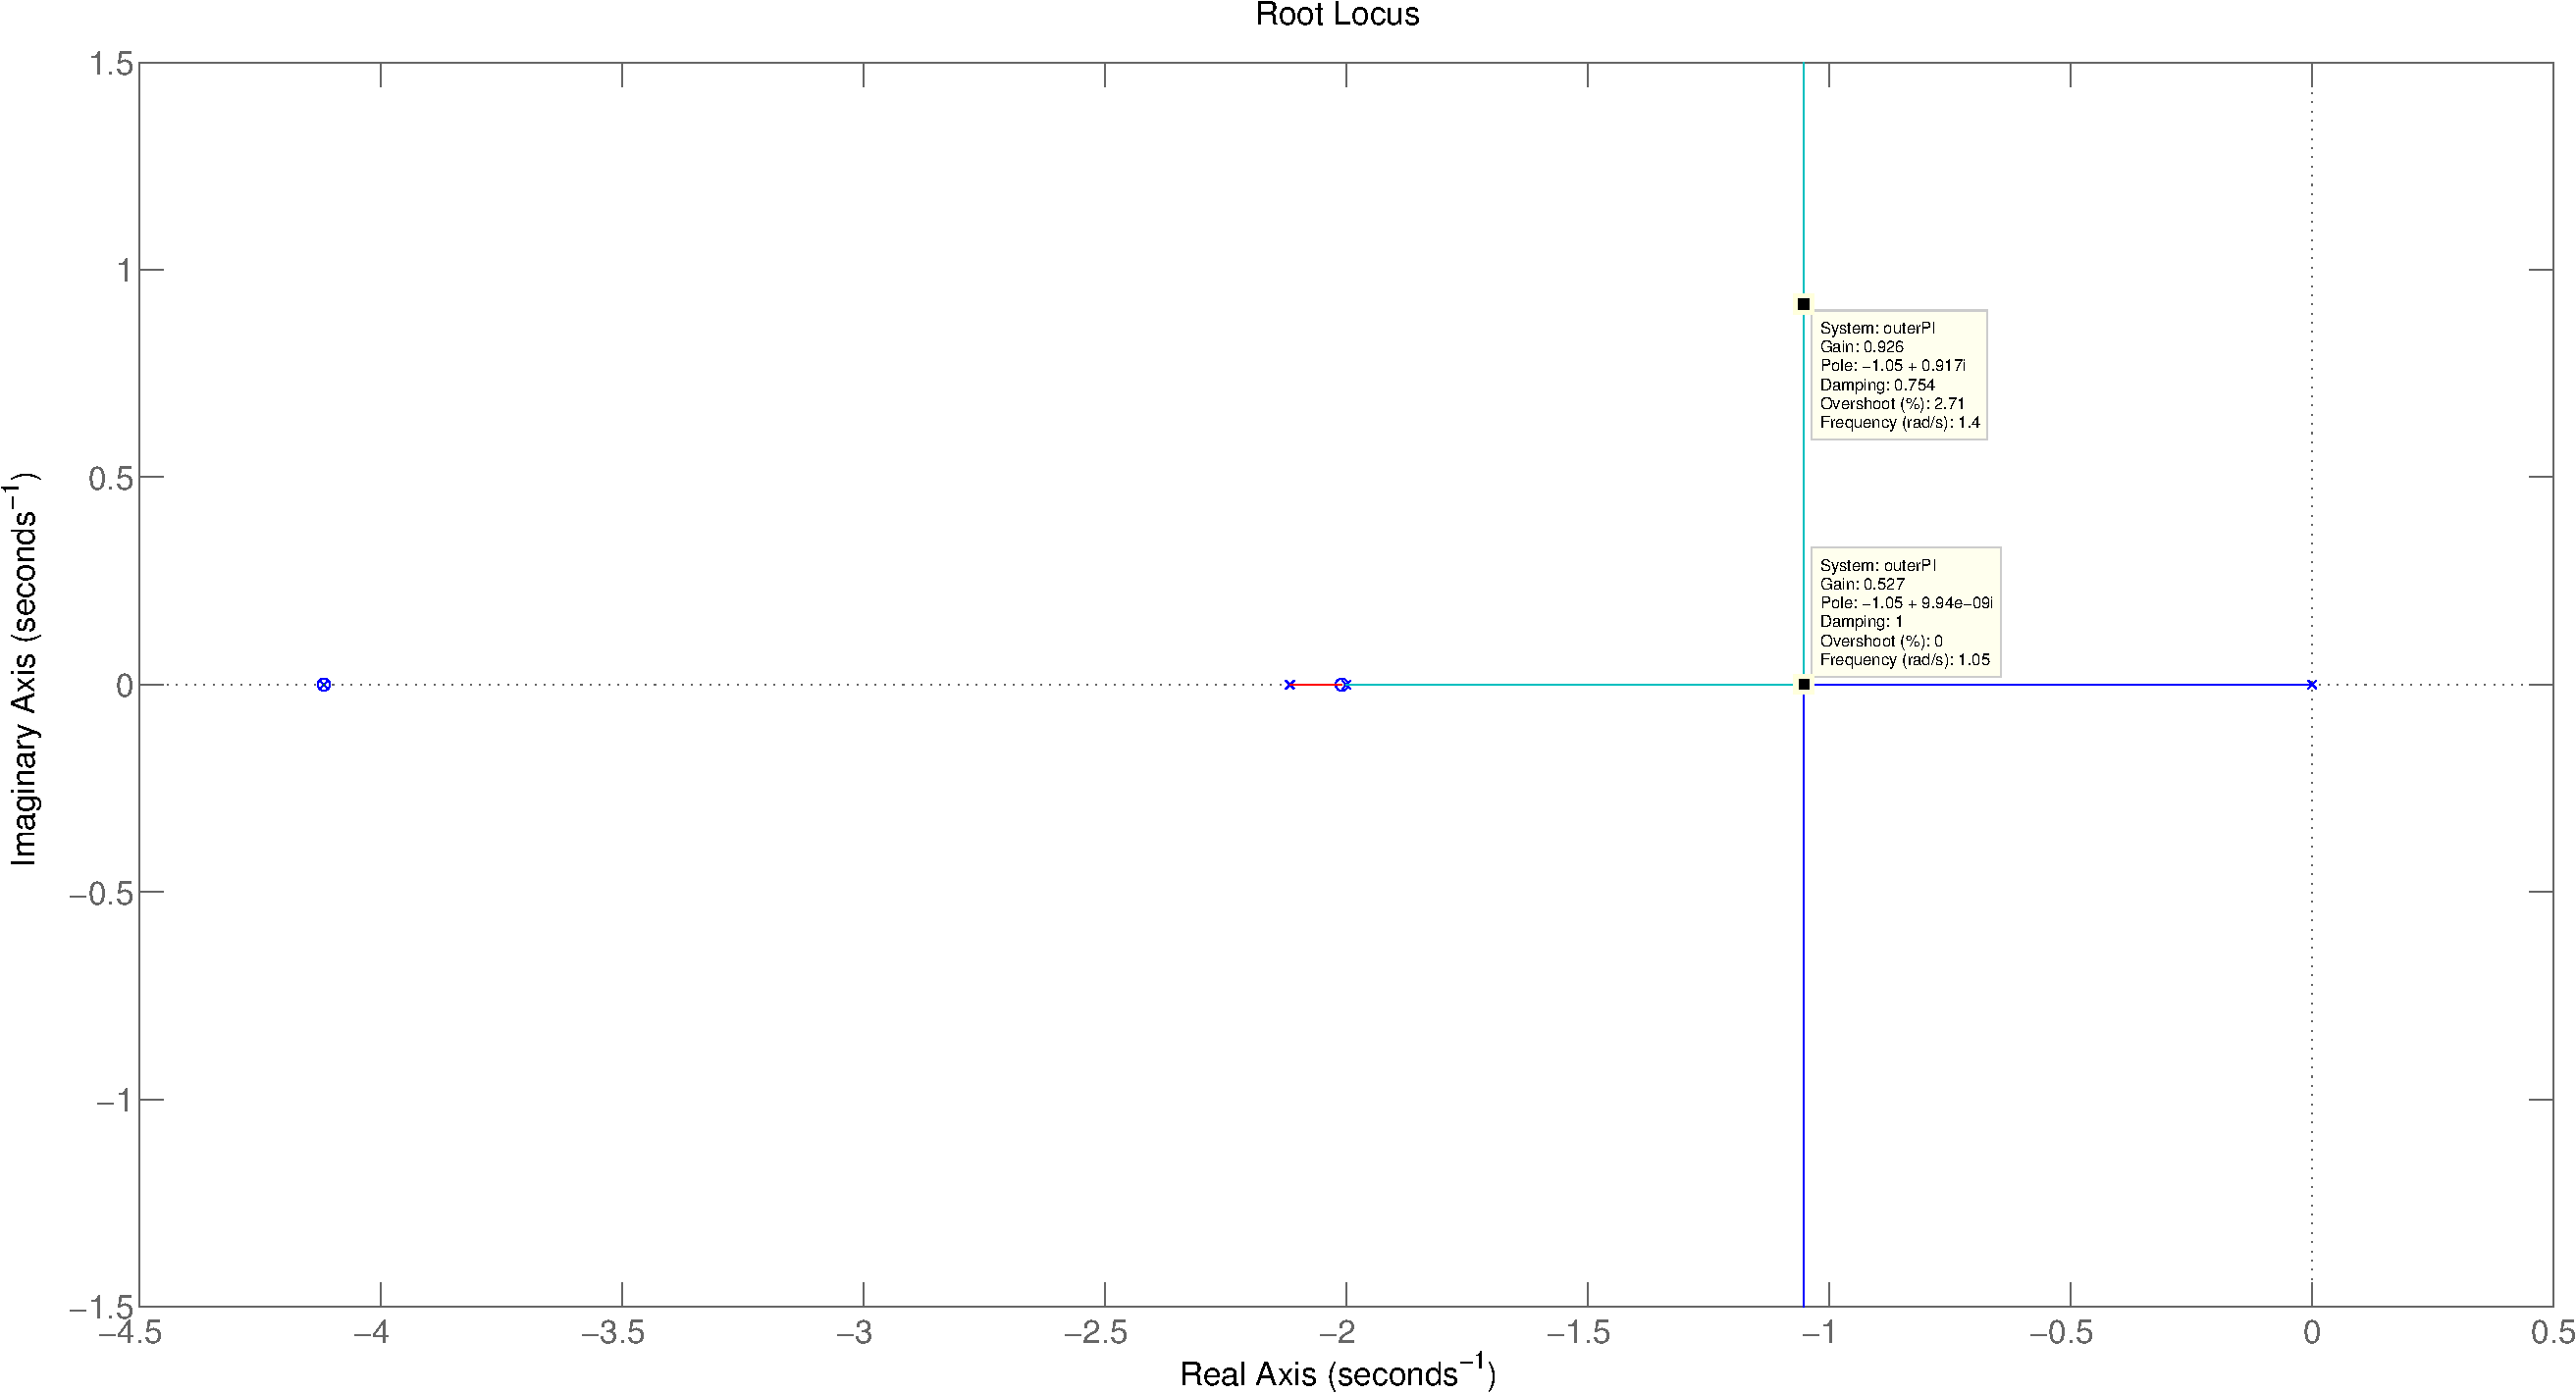
\includegraphics[width = \textwidth]{rlocus_outerTrac.pdf}
  \caption{Root locus of the outer traction loop\label{fig:rlocus_OuterTrac}}
\end{figure}
From the root locus, we can extract two reasonable first values: ${K_p}_{outer} \lessapprox 0.52$ would provide the fastest real poles and ${K_p}_{outer} \approx 0.93$ would provide a damping of $0.7$ -- any value inbetween could also be a good first choice. $K_i$ is then determined accordingly using $K_i = |z_{PI}| \cdot {K_P}_{outer}$. The root locus also shows us that if the poles of the inner loop are not perfectly known and $z_{PI}$ cannot be placed perfectly, ${p_{inner}}_{fast}<\nobreak z_{PI}<\nobreak{p_{inner}}_{slow}$ is better than ${p_{inner}}_{fast}<\nobreak{p_{inner}}_{slow}<\nobreak z_{PI}$
, because the latter pole-zero configuration would make the closed loop poles leave the real axis, as shown in figure \ref{fig:rlocus_outerTrac_bad}.
\begin{figure}[htbp]
  \centering
  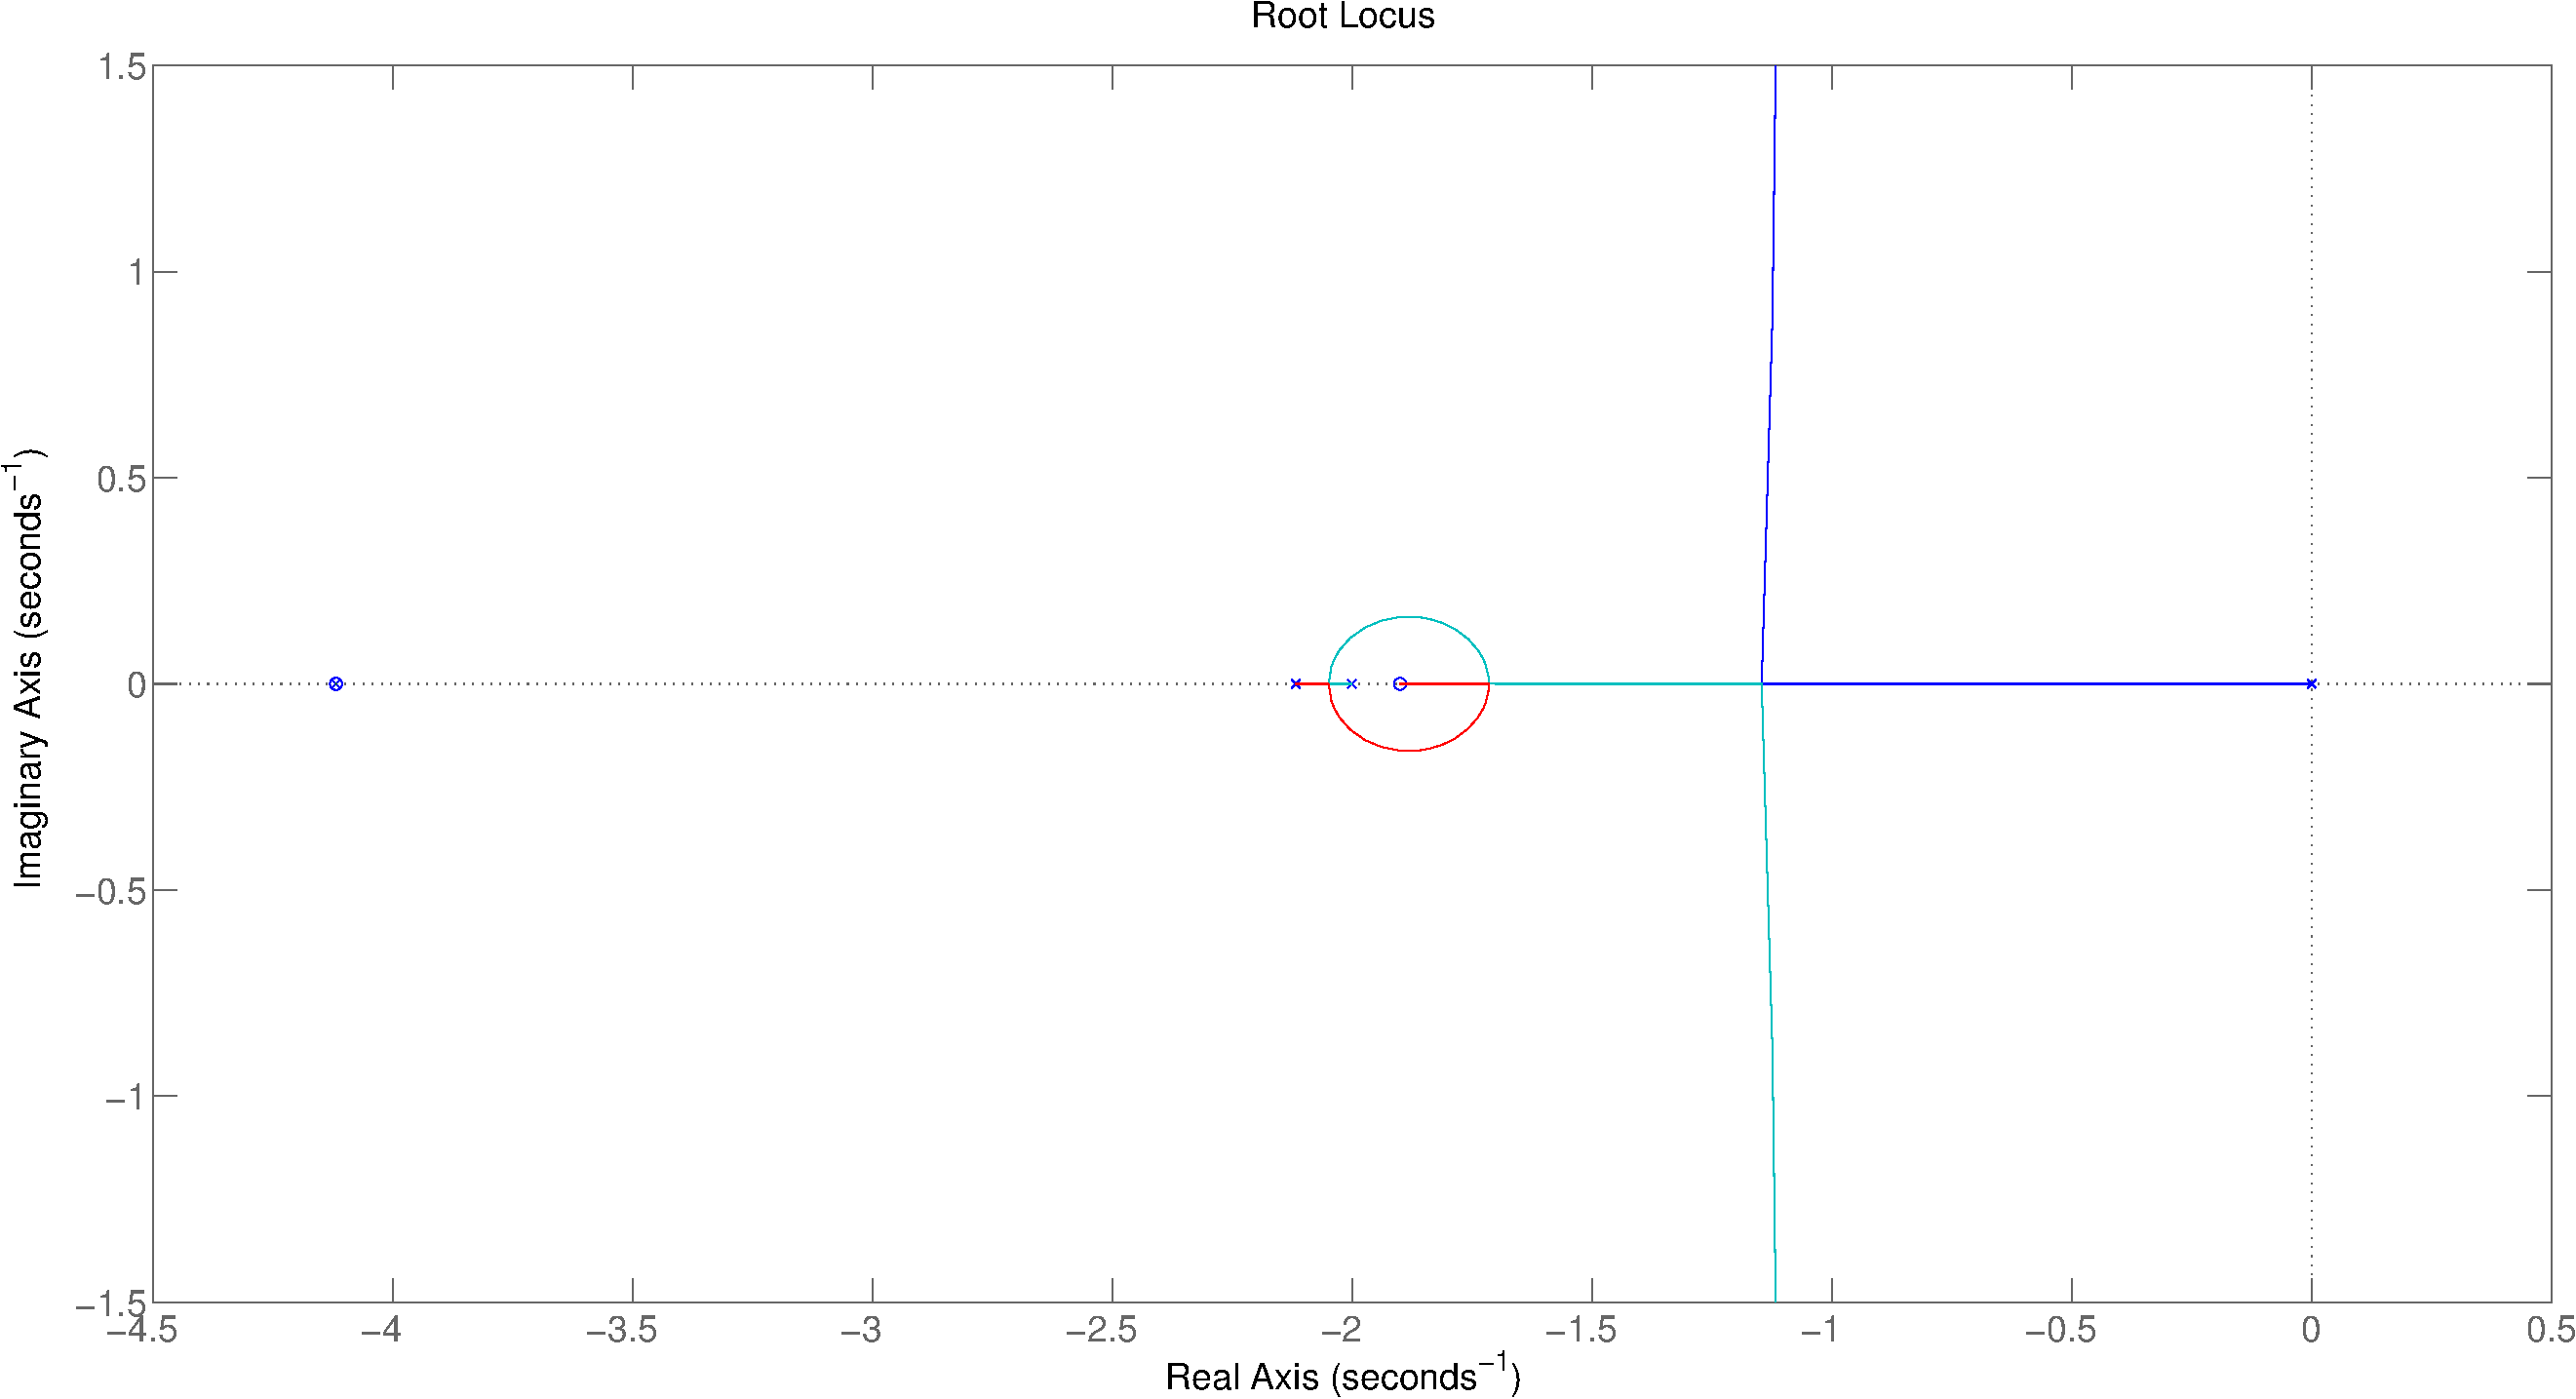
\includegraphics[width = .8\textwidth]{rlocus_outerTrac_bad.pdf}
  \caption{Root locus of the outer traction loop with a bad pole-zero configuration\label{fig:rlocus_outerTrac_bad}}
\end{figure}

With this controller, we should be able to move the integrating pole from the plant to the controller. The total closed loop should thus be stable and have zero steady-state error, perturbation rejection and a reasonable phase margin. In the following section, we will verify this design using simulink simulations and real world experiences and tune the gains if necessary.

\section{Tuning of the PI Controller}
Figure~\ref{fig:simu_tot_k06}
\begin{figure}[htbp]
  \centering
  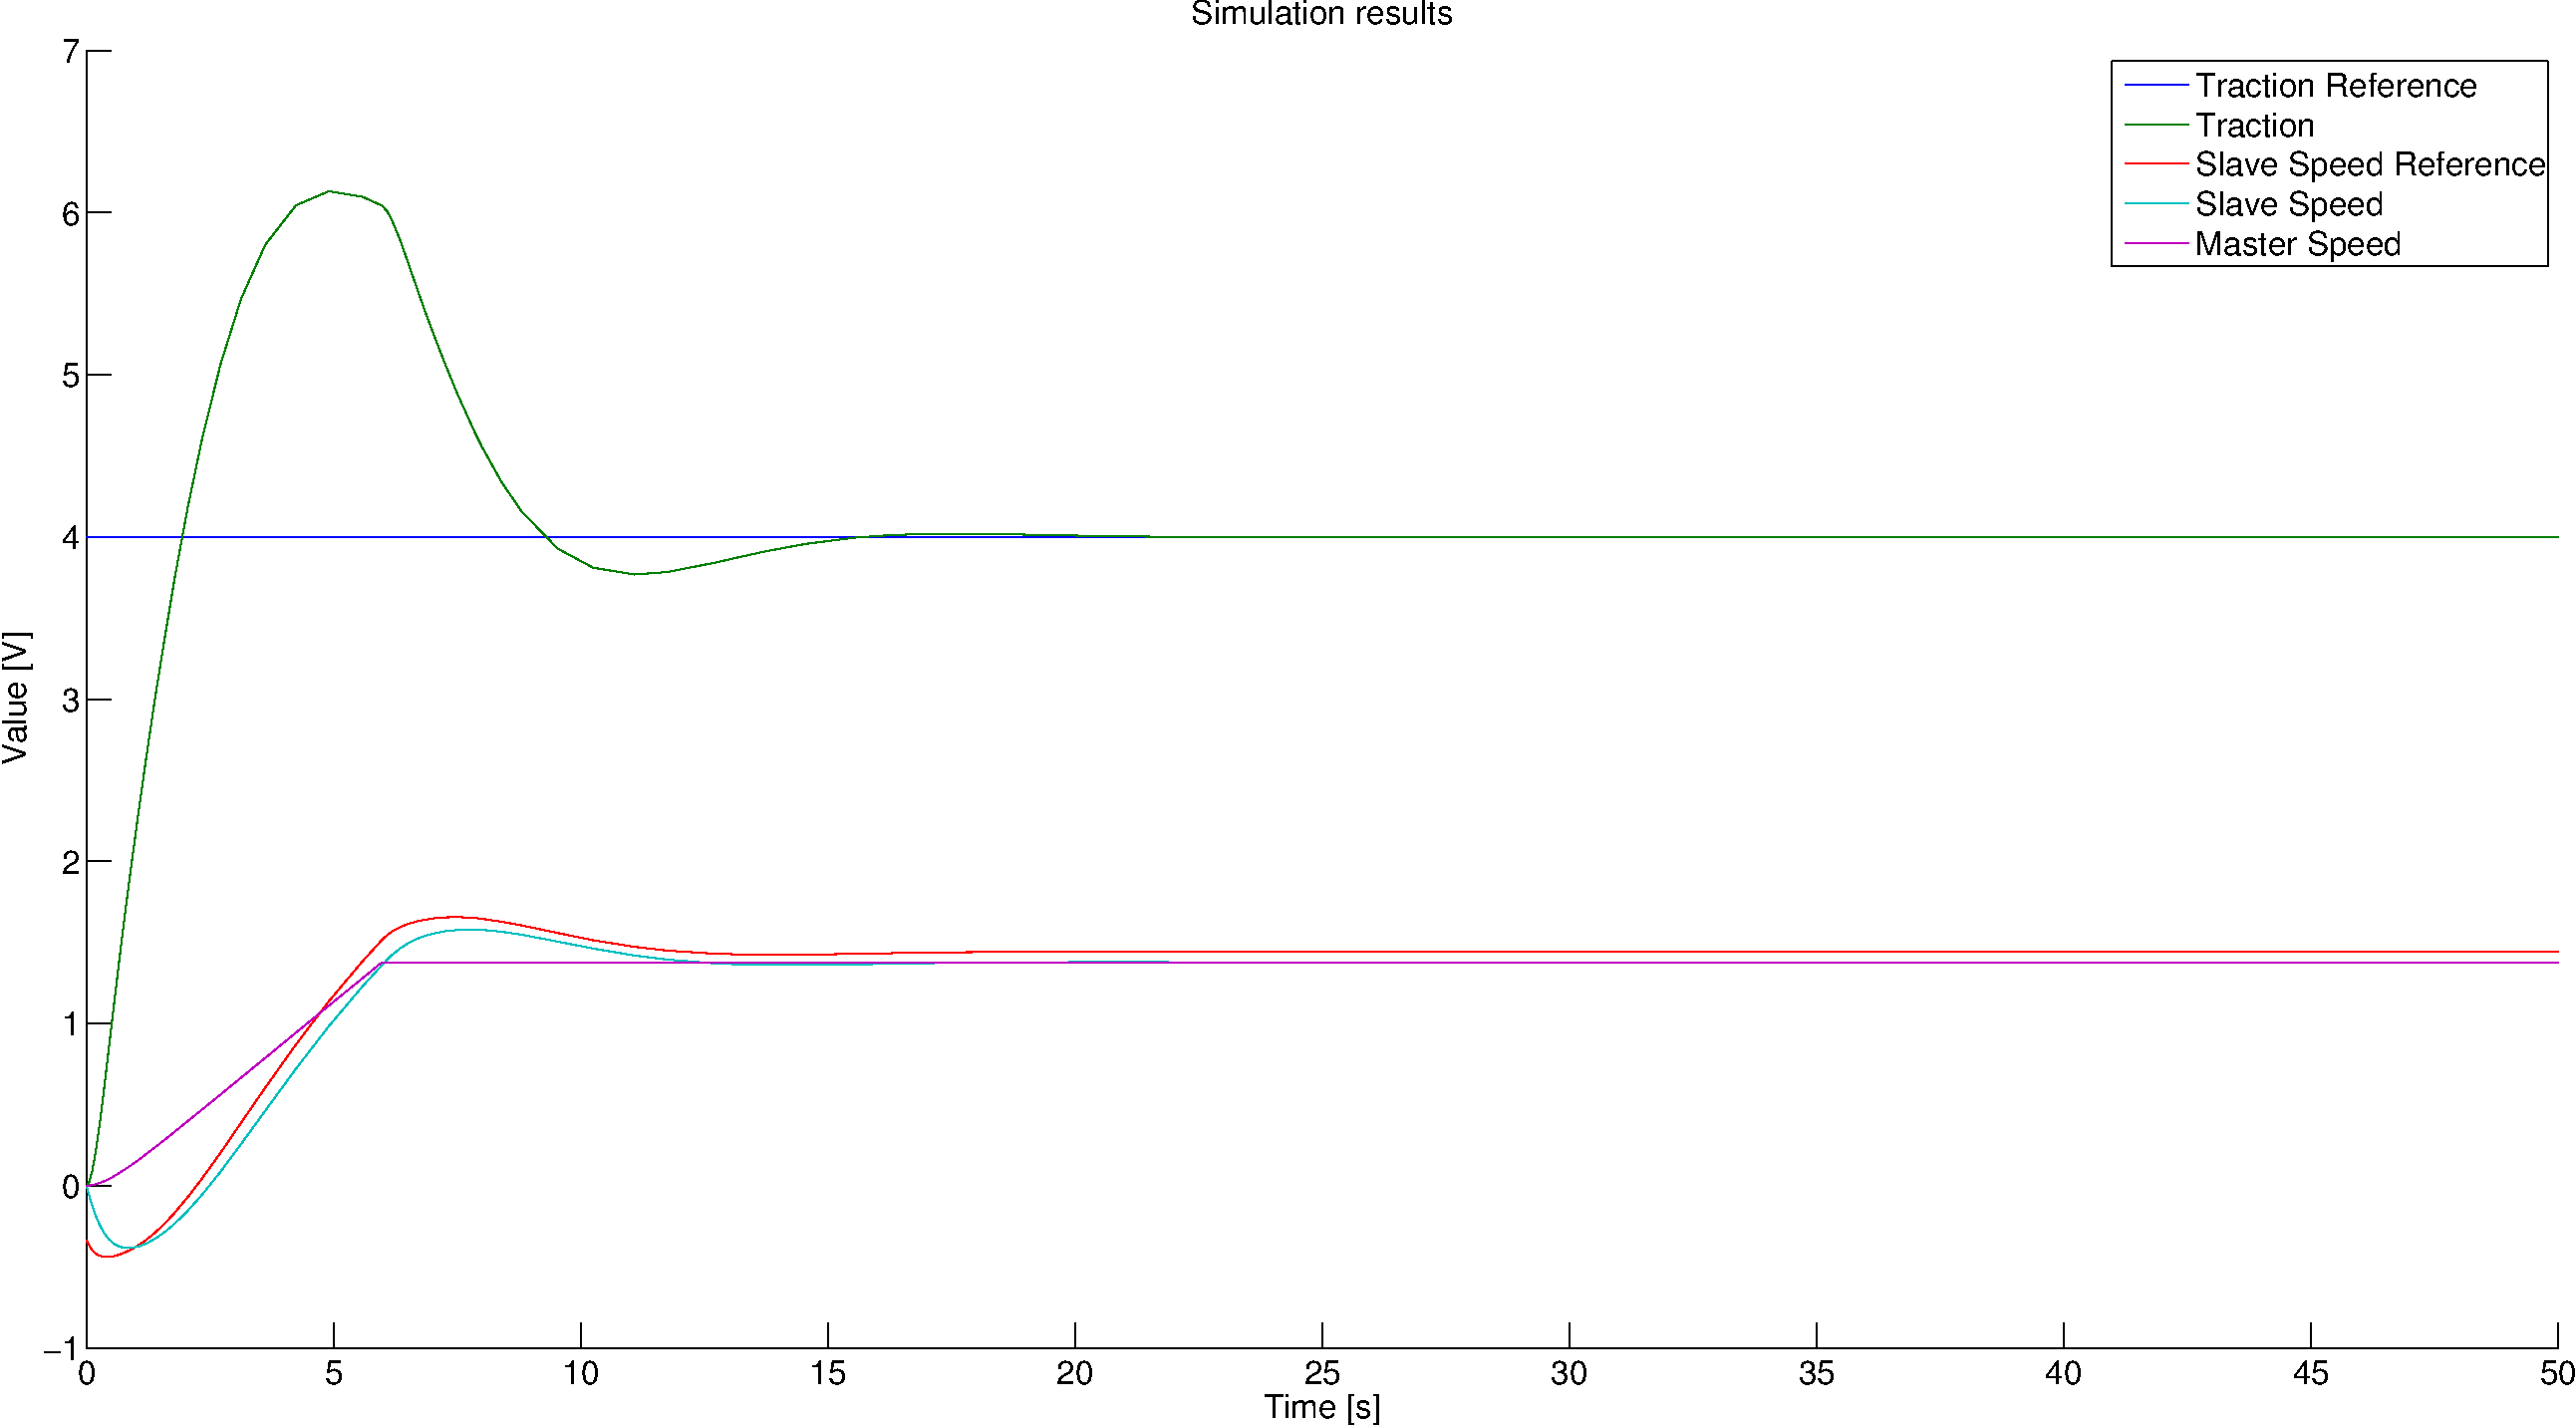
\includegraphics[width = \textwidth]{simu_tot_k06.pdf}
  \caption{Simulation of the rolling mill operation with a P - PI controller on the traction. ${K_p}_{outer} = 0.6$.\label{fig:simu_tot_k06}}
\end{figure}
shows the the simulated output of the rolling mill with the following gains:
\begin{align*}
  {K_p}_{inner} &= -0.14\\
  {K_p}_{outer} &= 0.6\\
  K_i &= 1.26
\end{align*}

We see that all the desired properties are achieved. However, the effect of the master speed ramp is still present, which is normal since a single integrator in the controller is able to reject perturbation of order $\leq 1$. This is supported by the experience, as shown in figure~\ref{fig:totalOut_k_0327_t_3}.
\begin{figure}[htbp]
  \centering
  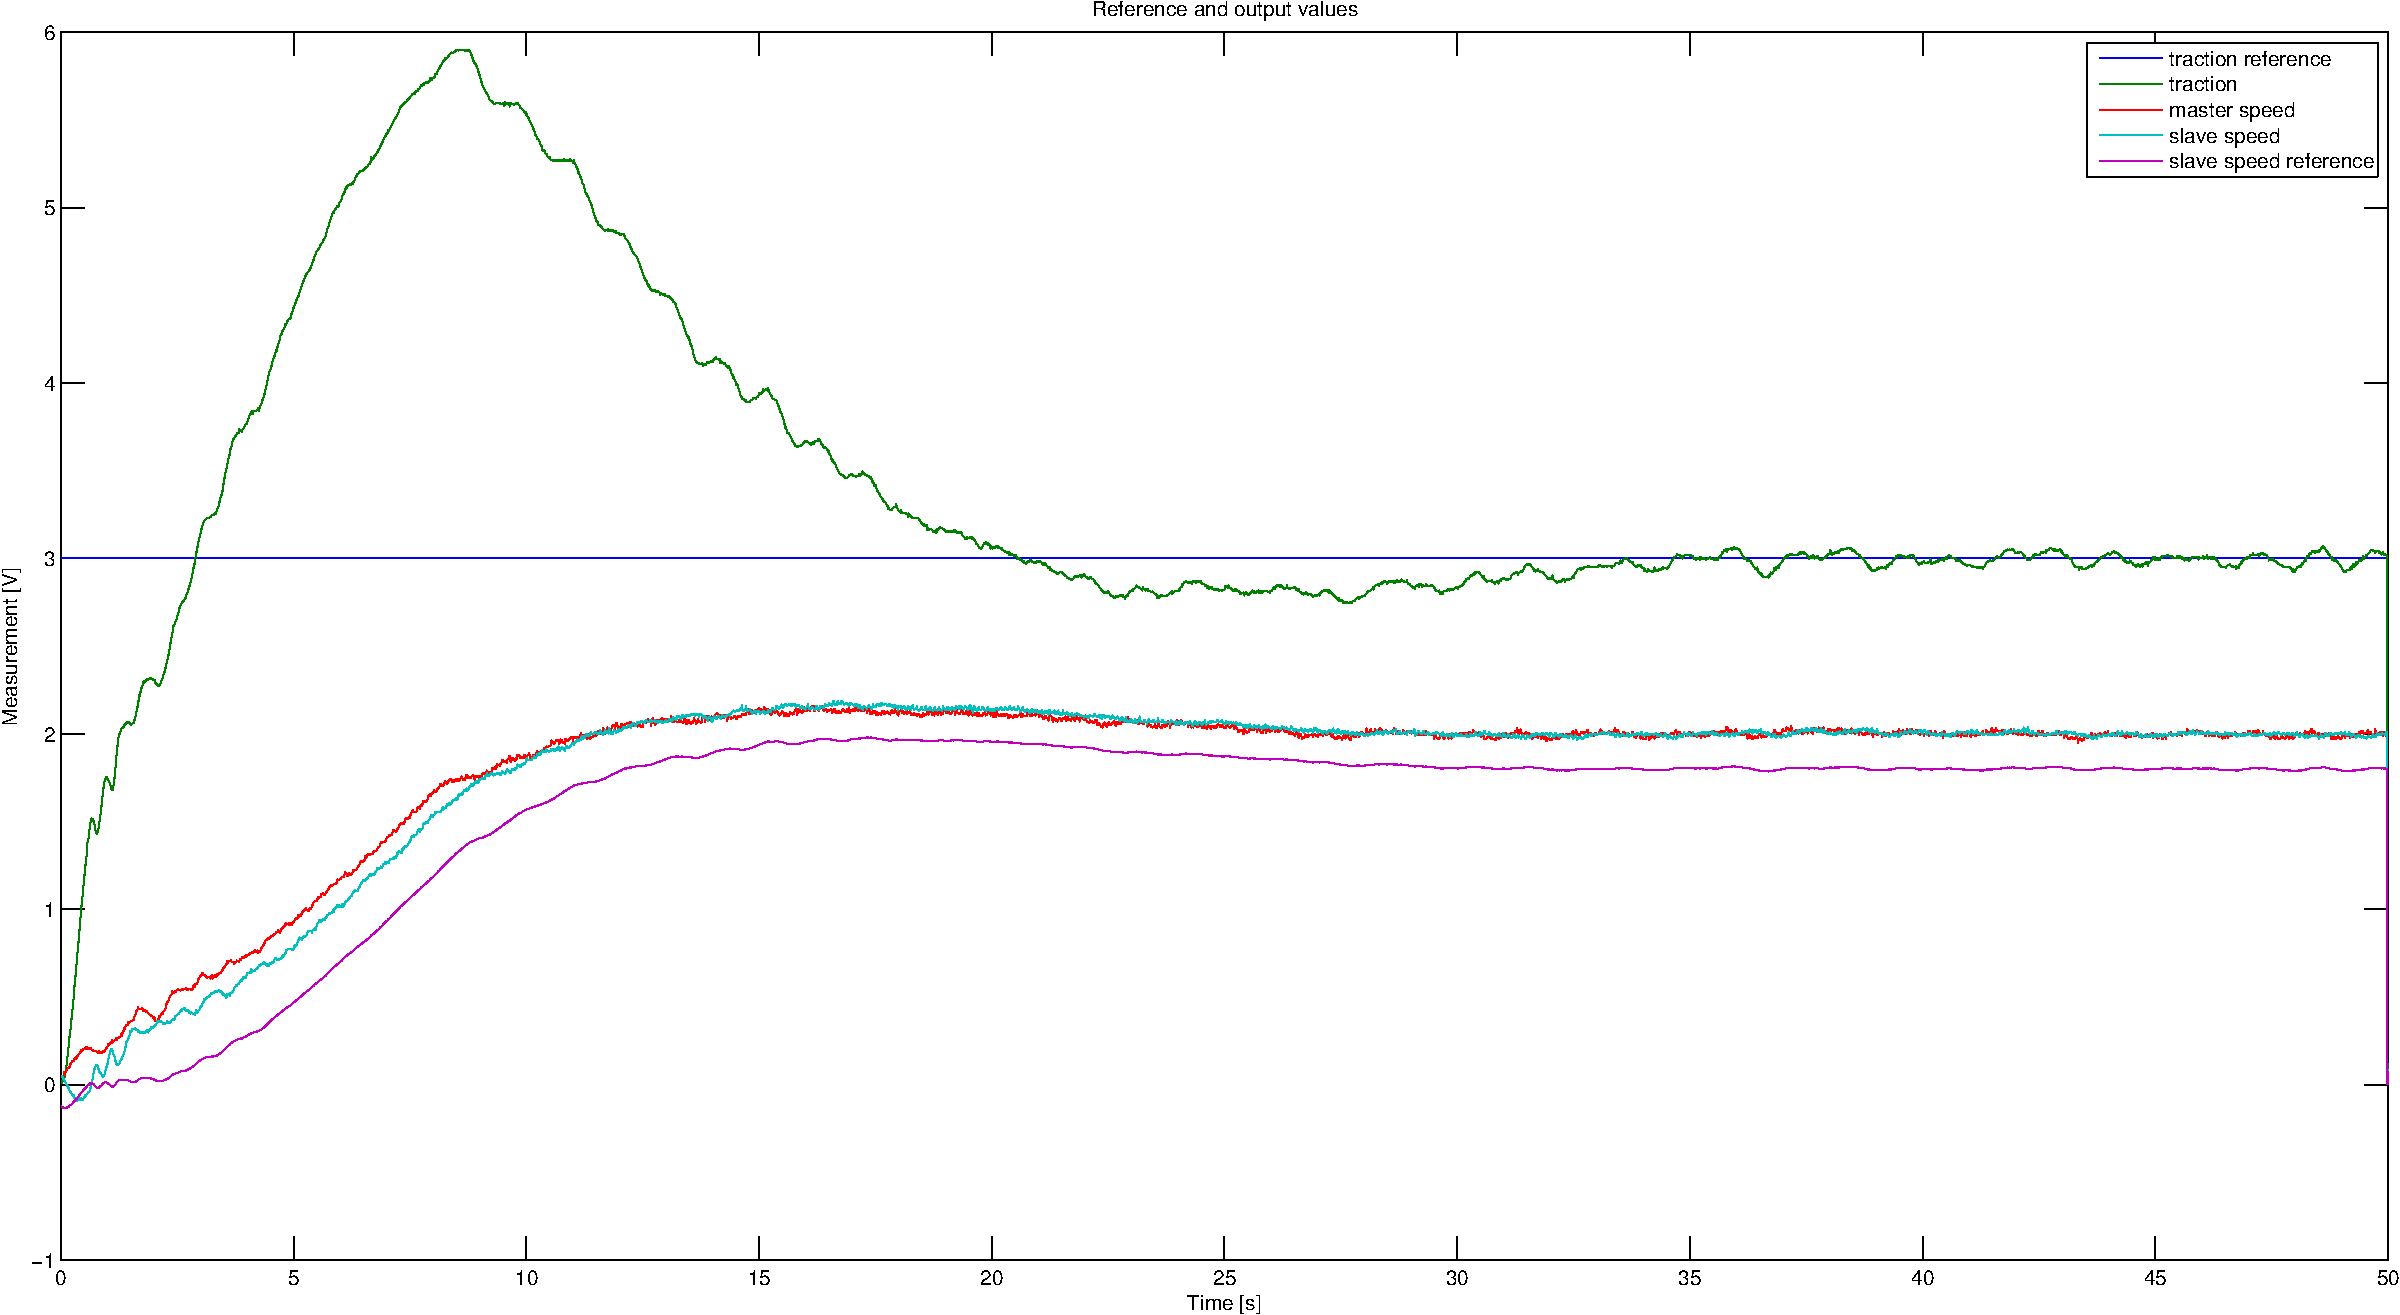
\includegraphics[width = \textwidth]{totalOut_k_0327_t_3.pdf}
  \caption{Operation of the rolling mill. ${K_p}_{outer} = 0.327$.\label{fig:totalOut_k_0327_t_3}}
\end{figure}

As a result, the controller should be tuned first and foremost to limit the overshoot induced by the initial ramp, because a measured traction $>\nobreak\SI{6}{V}$ is dangerous for the plant. We should thus increase ${K_P}_{outer}$ until the traction overshoot is low enough, and then check if the resulting lower damping is still satisfying.

Fortunately, figure~\ref{fig:totalOut_k_2_t_3}
\begin{figure}[htbp]
  \centering
  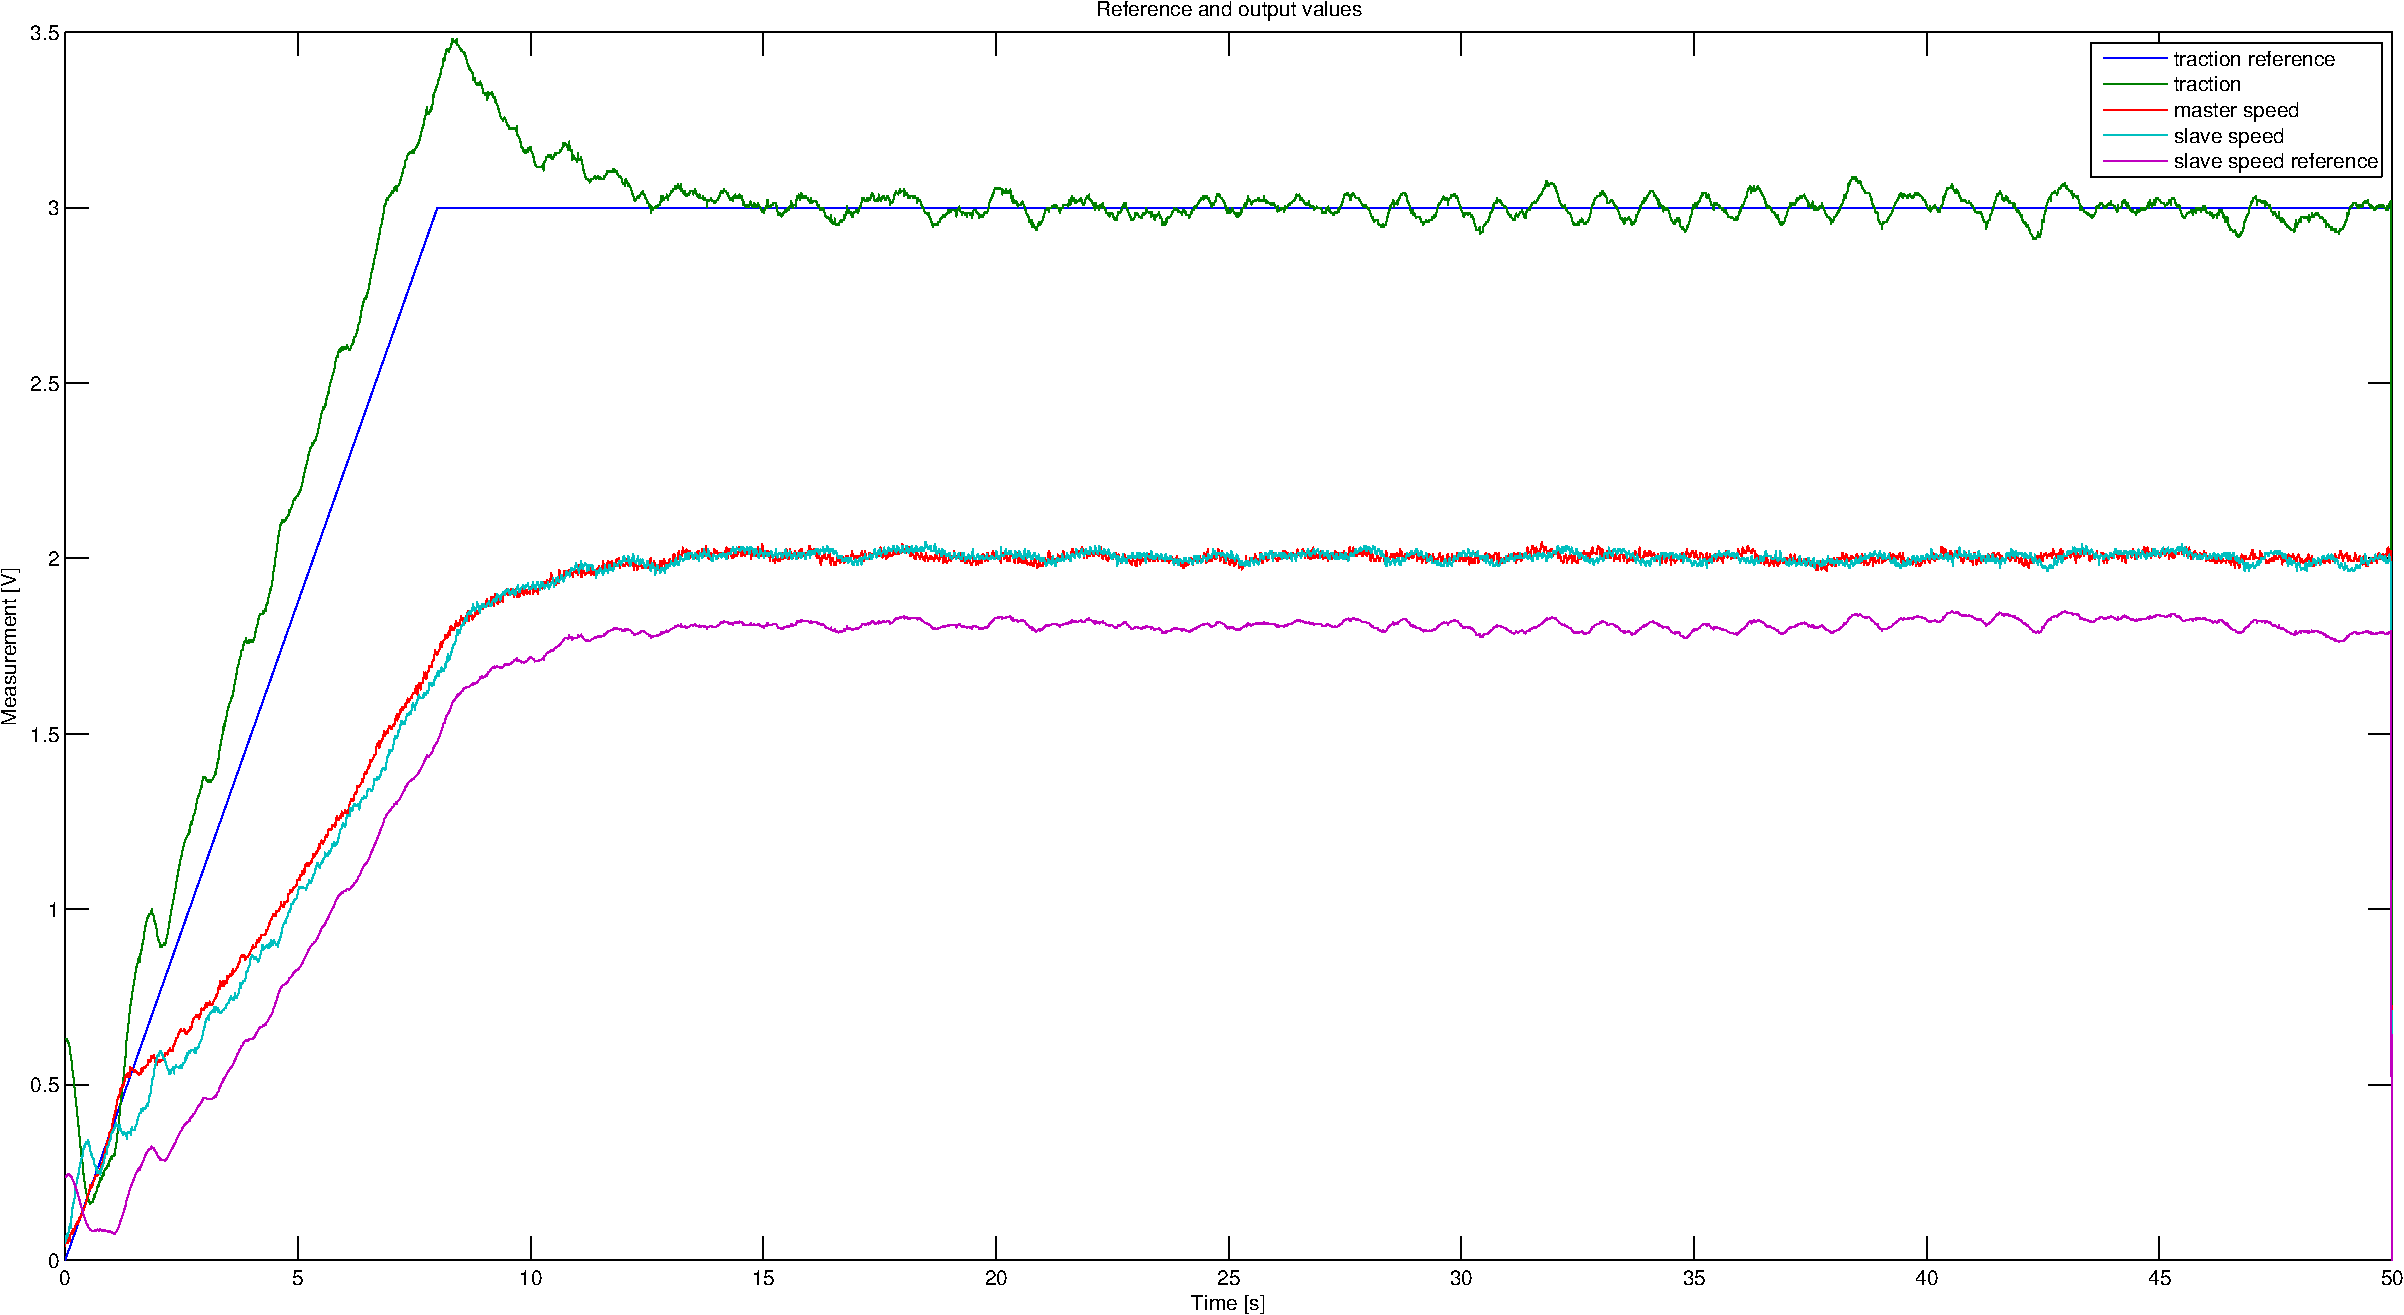
\includegraphics[width = \textwidth]{totalOut_k_2_t_3_ramp.pdf}
  \caption{Operation of the rolling mill. ${K_p}_{outer} = 2$.\label{fig:totalOut_k_2_t_3}}
\end{figure}
shows that values \ref{eqn:final_begin} - \ref{eqn:final_end}
\begin{figure*}[htb]
\begin{align}
  {K_p}_{inner} &= -0.14\label{eqn:final_begin}\\
  {K_p}_{outer} &= 2\\
  K_i &= 4.2\label{eqn:final_end}
\end{align}
\end{figure*}
along with an initial ramp on the traction provide an acceptable overshoot and sufficient damping. Figure~\ref{fig:totalCurr_k_2_t_3_ramp}
\begin{figure}[htbp]
  \centering
  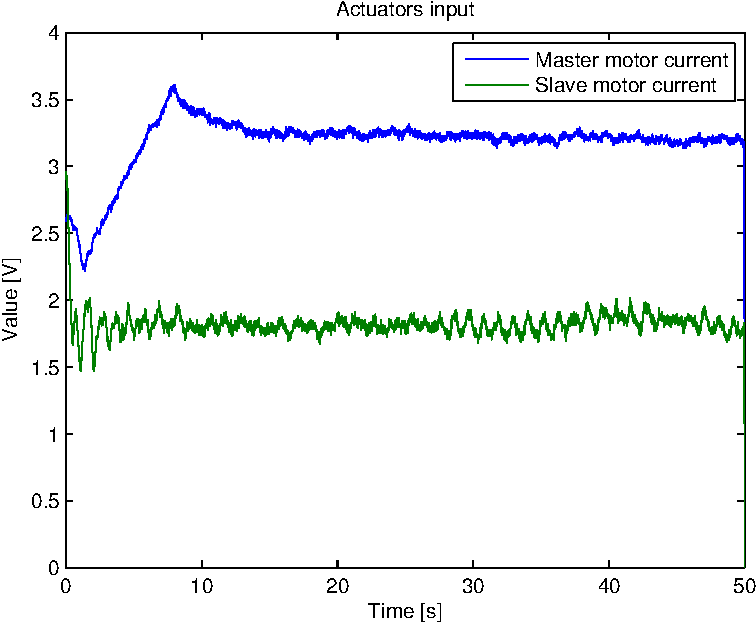
\includegraphics[width = \textwidth]{totalCurr_k_2_t_3_ramp.pdf}
  \caption{Actuators values during operation with the final controller\label{fig:totalCurr_k_2_t_3_ramp}}
\end{figure}
finishes the validation of this design by showing that the actuators do not go into saturation and are reasonably sollicitated during normal operation.

